% Created 2020-05-12 Tue 17:32
% Intended LaTeX compiler: pdflatex
\documentclass[11pt]{article}
\usepackage[utf8]{inputenc}
\usepackage[T1]{fontenc}
\usepackage{graphicx}
\usepackage{grffile}
\usepackage{longtable}
\usepackage{wrapfig}
\usepackage{rotating}
\usepackage[normalem]{ulem}
\usepackage{amsmath}
\usepackage{textcomp}
\usepackage{amssymb}
\usepackage{capt-of}
\usepackage{hyperref}
\usepackage{minted}
\usepackage{amsmath}
\usepackage{esint}
\usepackage[english, russian]{babel}
\usepackage{mathtools}
\usepackage{amsthm}
\usepackage[top=0.8in, bottom=0.75in, left=0.625in, right=0.625in]{geometry}
\usepackage{svg}
\usepackage{dot2texi}
\usepackage{tikz}
\usetikzlibrary{shapes, arrows, positioning}
\def\zall{\setcounter{lem}{0}\setcounter{cnsqnc}{0}\setcounter{th}{0}\setcounter{Cmt}{0}\setcounter{equation}{0}}
\newcounter{lem}\setcounter{lem}{0}
\def\lm{\par\smallskip\refstepcounter{lem}\textbf{\arabic{lem}}}
\newtheorem*{Lemma}{Лемма \lm}
\newcounter{th}\setcounter{th}{0}
\def\th{\par\smallskip\refstepcounter{th}\textbf{\arabic{th}}}
\newtheorem*{Theorem}{Теорема \th}
\newcounter{cnsqnc}\setcounter{cnsqnc}{0}
\def\cnsqnc{\par\smallskip\refstepcounter{cnsqnc}\textbf{\arabic{cnsqnc}}}
\newtheorem*{Consequence}{Следствие \cnsqnc}
\newcounter{Cmt}\setcounter{Cmt}{0}
\def\cmt{\par\smallskip\refstepcounter{Cmt}\textbf{\arabic{Cmt}}}
\newtheorem*{Note}{Замечание \cmt}
\author{Sergey Makarov}
\date{\today}
\title{}
\hypersetup{
 pdfauthor={Sergey Makarov},
 pdftitle={},
 pdfkeywords={},
 pdfsubject={},
 pdfcreator={Emacs 28.0.50 (Org mode 9.3)}, 
 pdflang={English}}
\begin{document}

\tableofcontents


\section{Семинар 1}
\label{sec:org3e72df2}
\subsection{Задача 1}
\label{sec:org1143517}
Построить СДНФ функции:
\begin{center}
\begin{tabular}{rrrr}
\hline
\(x_1\) & \(x_2\) & \(x_3\) & f\\
\hline
0 & 0 & 0 & 1\\
0 & 0 & 1 & 0\\
0 & 1 & 0 & 1\\
0 & 1 & 1 & 1\\
1 & 0 & 0 & 0\\
1 & 0 & 1 & 1\\
1 & 1 & 0 & 0\\
1 & 1 & 1 & 1\\
\hline
\end{tabular}
\end{center}
\subsubsection{Решение}
\label{sec:org98594a6}
   \begin{equation}
D_f^s(x_1, x_2, x_3) = \overline{x_1}\overline{x_2}\overline{x_3}\vee\overline{x_1}x_2\overline{x_3}
\vee\overline{x_1}x_2x_3\vee x_1\overline{x_2}x_3
   \end{equation}
\begin{equation}
K_f^s(x_1, x_2, x_3) = (x_1\vee x_2\vee\overline{x_3})(\overline{x_1}\vee x_2\vee x_3)
(\overline{x_1}\vee\overline{x_2}\vee x_3)(\overline{x_1}\vee\overline{x_2}\vee\overline{x_3})
\end{equation}
\subsection{Задача 2}
\label{sec:orgce4e38d}
  \begin{equation}
f = (00101111). \text{ Найти простые импликанты.}
  \end{equation}
\subsubsection{Решение}
\label{sec:org806d463}
   \begin{equation}
A = \{x_1, \overline{x_3}, x_1x_2, x_2\overline{x_3}\}\text{ - импликанты $f$.}
   \end{equation}
$x_1x_2$ - не простая импликанта.
\subsection{Задача 3}
\label{sec:orgaeec76d}
Найти простые импликанты функции
  \begin{equation}
f = (01111110).
  \end{equation}
\subsubsection{Решение}
\label{sec:org02d2d08}
   \begin{equation}
A = \{x_1\overline{x_2}, x_2x_3, x_1x_2x_3\}\text{ - импликанты}
   \end{equation}
$x_1\overline{x_2}$ - простая импликанта, $x_2x_3$ и $x_1x_2x_3$ - не импликанты.
\subsection{Задача 4}
\label{sec:orgbe17bb3}
Построить сокращённую ДНФ функции
\begin{equation}
\tilde{\alpha_f} = (1111 1000 0100 1100)
\end{equation}
\subsubsection{Решение}
\label{sec:orgda4f4c7}
Код максимальной грани: \((0022)\), соответствующая простая импликанта \(\overline{x_1}\overline{x^2}\).
Далее идёт ребро \((0200)\), соответствующее импликанте \(\overline{x_1}\overline{x_2}\overline{x_3}\).
Далее идёт ребро \((2100)\), соответствующее импликанте \(x_2\overline{x_3}\overline{x_4}\).
Следующее ребро \((1102) \rightarrow x_1x_2\overline{x_3}\),
\((1201) \rightarrow x_1\overline{x_3}x_4\), \((2001) \rightarrow \overline{x_2}\overline{x_3}x_4\).
\subsection{Задача 2.6}
\label{sec:orgd01971e}
Найти сокращённую ДНФ методом карты:
\begin{equation}
\tilde{\alpha_f} = (0101 0111)
\end{equation}
\subsubsection{Решение}
\label{sec:orgab0eb9c}
\begin{center}
\begin{tabular}{rrr}
\hline
x\textsubscript{1x}\textsubscript{2x}\textsubscript{3} & 0 & 1\\
\hline
00 & 0 & 1\\
01 & 0 & 1\\
11 & 1 & 1\\
10 & 0 & 1\\
\hline
\end{tabular}
\end{center}
Откуда \(D_f = x_3\vee x_1x_2\).
\subsection{Задача 2.6(5)}
\label{sec:org1b5d7fd}
  \begin{equation}
\tilde{\alpha_f} = (0001 1011 1101 1111)
  \end{equation}
\subsubsection{Решение}
\label{sec:orgc5bcc4b}
\begin{center}
\begin{tabular}{rrrrr}
\hline
\(x_1\) & \(x_2\) & \(x_3\) & \(x_4\) & \(f\)\\
\hline
0 & 0 & 0 & 0 & 0\\
0 & 0 & 0 & 1 & 0\\
0 & 0 & 1 & 0 & 0\\
0 & 0 & 1 & 1 & 1\\
0 & 1 & 0 & 0 & 1\\
0 & 1 & 0 & 1 & 0\\
0 & 1 & 1 & 0 & 1\\
0 & 1 & 1 & 1 & 1\\
1 & 0 & 0 & 0 & 1\\
1 & 0 & 0 & 1 & 1\\
1 & 0 & 1 & 0 & 0\\
1 & 0 & 1 & 1 & 1\\
1 & 1 & 0 & 0 & 1\\
1 & 1 & 0 & 1 & 1\\
1 & 1 & 1 & 0 & 1\\
1 & 1 & 1 & 1 & 1\\
\hline
\end{tabular}
\end{center}
Тогда карта Карно будет иметь вид:
\begin{center}
\begin{tabular}{rrrrrl}
\hline
\(x_1x_2x_3x_4\) & 00 & 01 & 11 & 10 & \\
\hline
00 & 0 & 0 & 1 & 0 & \(x_2x_3, x_2\overline{x_4}\)\\
01 & 1 & 0 & 1 & 1 & \(x_1x_2, x_1\overline{x_3}\)\\
11 & 1 & 1 & 1 & 1 & \(x_1x_4\)\\
10 & 1 & 1 & 1 & 0 & \(x_3x_4\)\\
\hline
\end{tabular}
\end{center}
Тогда сокращённая ДНФ имеет вид:
\begin{equation}
D_f = x_2\overline{x_4}\vee x_2x_3\vee x_1x_2\vee x_1x_4\vee x_3x_4\vee x_1\overline{x_3}
\end{equation}
\subsection{Задача 2.3(1)}
\label{sec:org3eed672}
Получить сокращённую ДНФ по КНФ:
\begin{equation}
(x_1\vee x_2\vee\overline{x_3})(\overline{x_1}\vee x_2\vee x_3)(\overline{x_2}\vee\overline{x_3})
\end{equation}
\subsubsection{Решение}
\label{sec:org00e7023}
\begin{multline}
   (x_1\vee x_2\vee\overline{x_3})(\overline{x_1}\vee x_2\vee x_3)(\overline{x_2}\vee\overline{x_3})
= (x_1x_2\vee x_1x_3 \vee x_2\overline{x_1}\vee x_2\vee x_2x_3\vee\overline{x_1}\overline{x_3}
\vee x_2\overline{x_3})(\overline{x_2}\vee\overline{x_3}) = \\
= (x_2\vee x_1x_3\vee\overline{x_1}\overline{x_3})(\overline{x_2}\vee\overline{x_3})
= x_2\overline{x_3}\vee x_1\overline{x_2}x_3\vee\overline{x_1}\overline{x_2}\overline{x_3}
\vee\overline{x_1}\overline{x_3} = x_2\overline{x_3}\vee\overline{x_1}\overline{x_3}\vee x_1\overline{x_2}x_3
\end{multline}
\subsection{Задача 2.2(1)}
\label{sec:org90e6f3f}
Построить сокращённую ДНФ по данной ДНФ методом Блейка:
\begin{equation}
\overline{x_1}\overline{x_2}\vee x_1\overline{x_2}x_4\vee x_2\overline{x_3}x_4\vee\overline{x_2}x_4|
\vee\overline{x_1}\overline{x_3}x_4\vee x_1\overline{x_3}x_4|\vee\overline{x_2}\overline{x_3}x_4
\vee\overline{x_3}x_4 = \overline{x_1}\overline{x_2}\vee\overline{x_2}x_4\vee\overline{x_3}x_4
\end{equation}
\subsection{Задача 2.2(2)}
\label{sec:org782a3f4}
  \begin{equation}
x_1\overline{x_2}x_3\vee\overline{x_1}x_2\overline{x_4}\vee\overline{x_2}\overline{x_3}x_4|
\vee x_1\overline{x_2}x_4
  \end{equation}
\subsection{Задача 2.9(1)}
\label{sec:orga2885c2}
  \begin{equation}
f(\tilde{x_n}) = x_1\oplus\ldots\oplus x_n
  \end{equation}
Длина сокращённой ДНФ - ?
\subsubsection{Решение}
\label{sec:orgbd2cc7c}
   Максимальные грани - точки $\Rightarrow$ длина сокращённой ДНФ, она же длина СДНФ равна
$2^n - 1$.
\subsection{Задача 2.9(2)}
\label{sec:orged908cb}
Найти длину сокращённой ДНФ функции:
  \begin{equation}
f(\tilde{x_n}) = (x_1\vee x_2\vee x_3)(\overline{x_1}\vee\overline{x_2}\overline{x_3})\oplus
x_4\oplus\ldots\oplus x_n
  \end{equation}
\subsubsection{Решение}
\label{sec:org9d006a8}
\begin{equation}
f(\tilde{\alpha}) = 1 \Leftrightarrow \begin{cases}
g(\tilde{\alpha}) = 1, \\
h(\tilde{\alpha}) = 0, \\
g(\tilde{\alpha}) = 0, \\
h(\tilde{\alpha}) = 1.
   \end{cases}
\end{equation}
Первому случаю соответствует $2^{n - 4}\cdot6$ максимальных грани, второму - $2\cdot2^{n - 4}$,
итого длина ДНФ составляет $2^{n - 1}$.

\url{http://mk.cs.msu.ru}, лекционные курсы, ОКи, домашние задания там.
\section{Домашняя работа 1}
\label{sec:orgec09ba4}
\subsection{Задача 2.3(4)}
\label{sec:orgdc3ab74}
Представить в виде СДНФ функцию:
\zall
\begin{equation}
f(\tilde{x}^3) = (01010001)
\end{equation}
\subsubsection{Решение}
\label{sec:orgb3a21e7}
Функция принимает единичные значения на наборах $001, 011$ и $111$, откуда СДНФ имеет вид:
\begin{equation}
f(\tilde{x}^3) = \overline{x_1}\overline{x_2}x_3\vee\overline{x_1}x_2x_3\vee x_1x_2x_3
\end{equation}
\subsection{Задача 2.1(3)}
\label{sec:org82c0d97}
Из множества \(A\) ЭК выделить простые импликанты функции \(f\):
\begin{equation}
A = \{x_1, \overline{x_4}, x_2\overline{x_3}, \overline{x_1}\overline{x_2}\overline{x_4}\},
f(\tilde{x}^4) = (1010 1110 1101 1110)
\end{equation}
\subsubsection{Решение}
\label{sec:org482a460}
ЭК $x_1$ не является импликантой функции $f$, так как $f(1111) = 0$.

ЭК $\overline{x_4}$ является простой импликантой функции $f$.

ЭК $x_2\overline{x_3}$ является импликантой функции $f$. ЭК $x_2$ не является импликантой
функции $f$, так как $f(1111) = 0$. ЭК $\overline{x_3}$ также не является импликантой $f$,
так как $f(0001) = 0$, значит $x_2\overline{x_3}$ -- простая импликанта функции $f$.

ЭК $\overline{x_1}\overline{x_2}\overline{x_4}$ является импликантой функции $f$, но она не
является простой, так как содержит множитель $\overline{x_4}$, который, как было указано ранее,
является импликантой $f$.
\subsection{Задача 2.5(2, 6)}
\label{sec:org4dbb9b9}
Изобразив множество \(N_f\) функции \(f(\tilde{x}^n)\) в \(B^n\), найти коды максимальных интервалов
и построить сокращённую ДНФ:
\begin{equation}
\tilde{\alpha}_f = (0101 0011)
\end{equation}
\begin{equation}
\tilde{\alpha}_f = (0001 0111 1110 1111)
\end{equation}
\subsubsection{Решение}
\label{sec:orgd7cdda9}
Для первой функции находим две максимальные грани с кодами \((112)\) и \((021)\), попытки расширить
которые приводят к выходу из \(N_f\). Отсюда получаем сокращённую ДНФ:
\begin{equation}
f(\tilde{x}^3) = \overline{x_1}x_3\vee x_1x_2
\end{equation}
Для второй функции максимальные грани имеют коды \((2112)\), \((1202)\), \((0121)\) и \((0211)\).
Попытки расширить эти грани приводят к выходу из \(N_f\). Отсюда получаем сокращённую ДНФ:
\begin{equation}
f(\tilde{x}^4) = x_2x_3\vee x_1\overline{x_3}\vee\overline{x_1}x_2x_4\vee\overline{x_1}x_3x_4
\end{equation}
\subsection{Задача 2.6(2, 6)}
\label{sec:org06dcc53}
Найти сокращённую ДНФ функции с помощью минимизирующей карты:
\begin{equation}
\tilde{\alpha_f} = (1101 1011)
\end{equation}
\begin{equation}
\tilde{\alpha_f} = (0011 1101 1111 1101)
\end{equation}
Карта Карно для первой функции:
\begin{center}
\begin{tabular}{rrrrr}
\hline
\(x_1\) $\backslash$ \(x_2x_3\) & 00 & 01 & 11 & 10\\
\hline
0 & 1 & 1 & 1 & 0\\
1 & 1 & 0 & 1 & 1\\
\hline
\end{tabular}
\end{center}
В данном случае максимальными по включению будут прямоугольники \((00-)\), \((-00)\), \((0-1)\),
\((-11)\), \((11-)\), \((1-0)\), откуда сокращённая ДНФ имеет вид:
\begin{equation}
f(\tilde{x}^3) = \overline{x_1}\overline{x_2}\vee\overline{x_2}\overline{x_3}\vee\overline{x_1}x_3
\vee x_2x_3\vee x_1x_2\vee x_1\overline{x_3}
\end{equation}
Карта Карно для второй функции:
\begin{center}
\begin{tabular}{rrrrr}
\hline
\(x_1x_2\) $\backslash$ \(x_3x_4\) & 00 & 01 & 11 & 10\\
\hline
00 & 0 & 0 & 1 & 1\\
01 & 1 & 1 & 1 & 0\\
11 & 1 & 1 & 1 & 0\\
10 & 1 & 1 & 1 & 1\\
\hline
\end{tabular}
\end{center}
Максимальными по включению здесь будут прямоугольники \((10--), (-10-), (--11), (-010)\),
которые дают сокращённую ДНФ:
\begin{equation}
f(\tilde{x}^4) = x_1\overline{x_2}\vee x_2\overline{x_3}\vee x_3x_4\vee\overline{x_2}x_3\overline{x_4}
\end{equation}
\subsection{Задача 2.2(3, 4)}
\label{sec:org1a84dee}
По заданной ДНФ методом Блейка получить сокращённую ДНФ:
\begin{equation}
D = x_1\vee\overline{x_1}x_2\vee\overline{x_1}\overline{x_2}x_3\vee\overline{x_1}x_2x_3x_4
\end{equation}
\begin{equation}
D = x_1\overline{x_2}x_4\vee\overline{x_1}\overline{x_2}x_3\vee\overline{x_3}\overline{x_4}
\end{equation}
\subsubsection{Решение}
\label{sec:org40c2e64}
\begin{multline}
x_1\vee\overline{x_1}x_2\vee\overline{x_1}\overline{x_2}x_3\vee\overline{x_1}x_2x_3x_4 = \\
= x_1\vee\overline{x_1}x_2\vee\overline{x_1}\overline{x_2}x_3\vee\overline{x_1}x_2x_3x_4
\vee x_2\vee\overline{x_2}x_3\vee x_2x_3x_4\vee\overline{x_1}x_3\vee\overline{x_1}x_3x_4 = \\
= x_1\vee x_2\vee\overline{x_1}x_3\vee\overline{x_2}x_3\vee
= x_1\vee x_2\vee\overline{x_1}x_3\vee\overline{x_2}x_3\vee x_3
= x_1\vee x_2\vee x_3
\end{multline}
\begin{multline}
x_1\overline{x_2}x_4\vee\overline{x_1}\overline{x_2}x_3\vee\overline{x_3}\overline{x_4}
= x_1\overline{x_2}x_4\vee\overline{x_1}\overline{x_2}x_3\vee\overline{x_3}\overline{x_4}\vee
\overline{x_2}x_3x_4\vee\overline{x_1}\overline{x_2}\overline{x_4}\vee x_1\overline{x_2}\overline{x_3} = \\
= x_1\overline{x_2}x_4\vee\overline{x_1}\overline{x_2}x_3\vee\overline{x_3}\overline{x_4}\vee
\overline{x_2}x_3x_4\vee\overline{x_1}\overline{x_2}\overline{x_4}\vee x_1\overline{x_2}\overline{x_3}\vee
\overline{x_2}\overline{x_3}\overline{x_4}\vee x_1\overline{x_2}x_4\vee\overline{x_1}\overline{x_2}x_3 = \\
= x_1\overline{x_2}x_4\vee\overline{x_1}\overline{x_2}x_3\vee\overline{x_3}\overline{x_4}
\vee\overline{x_2}x_3x_4\vee\overline{x_1}\overline{x_2}\overline{x_4}\vee x_1\overline{x_2}\overline{x_3}
\end{multline}
\subsection{Задача 2.3(3, 4)}
\label{sec:org996046e}
Построить сокращённую ДНФ по заданной КНФ:
\begin{equation}
(x_1\vee\overline{x_2}\vee\overline{x_3})(\overline{x_1}\vee x_2)(x_1\vee x_2\vee x_3)
\end{equation}
\begin{equation}
(x_1\vee x_2\vee x_3)(\overline{x_1}\vee\overline{x_2}\vee\overline{x_3})
\end{equation}
\subsubsection{Решение}
\label{sec:orgc70538b}
\begin{multline}
(x_1\vee\overline{x_2}\vee\overline{x_3})(\overline{x_1}\vee x_2)(x_1\vee x_2\vee x_3) =
(x_1x_2\vee\overline{x_1}\overline{x_2}\vee\overline{x_1}\overline{x_3}\vee x_2\overline{x_3})
(x_1\vee x_2\vee x_3) = \\
= x_1x_2\vee x_1x_2x_3\vee\overline{x_1}\overline{x_2}x_3\vee\overline{x_1}x_2\overline{x_3}\vee
x_1x_2\overline{x_3}\vee x_2\overline{x_3} = x_1x_2\vee x_2\overline{x_3}\vee\overline{x_1}\overline{x_2}x_3
\end{multline}
\begin{equation}
(x_1\vee x_2\vee x_3)(\overline{x_1}\vee\overline{x_2}\vee\overline{x_3})
= x_1\overline{x_2}\vee x_1\overline{x_3}\vee\overline{x_1}x_2\vee x_2\overline{x_3}\vee
\overline{x_1}x_3\vee\overline{x_2}x_3
\end{equation}
\subsection{Задача 2.9(6)}
\label{sec:org6d31ab6}
Найти длину сокращённой ДНФ функции \(f\):
\begin{equation}
f(\tilde{x}^n) = (x_1\vee\ldots\vee x_n)(x_1\vee\ldots\vee x_k\vee\overline{x}_{k + 1}\vee\ldots\vee\overline{x}_n)
\end{equation}
\subsubsection{Решение}
\label{sec:orge9b6440}
\begin{multline}
(x_1\vee\ldots\vee x_n)(x_1\vee\ldots\vee x_k\vee\overline{x}_{k + 1}\vee\ldots\overline{x}_n) =
(\vee_{i = 1}^kx_k)\vee(\vee_{i, j = 1}^{k, n}x_ix_j)\vee(\vee_{i = k + 1, j = 1}^{n}\overline{x}_ix_j) = \\
= (\vee_{i = 1}^kx_k)\vee(\vee_{i, j = k + 1}^n\overline{x_i}x_j)\vee(\vee_{i, j = k + 1}^nx_ix_j)
\end{multline}
Всего получаем
\begin{equation}
k + 2\frac{(n - k)(n - k + 1)}2 = k + (n - k)(n - k + 1) = n + (n - k)^2 = n^2 - 2nk + n + k^2
\end{equation}
слагаемых.
\section{Семинар 2}
\label{sec:org165568b}
\subsection{Задача 3.1(1, 5)}
\label{sec:org00244b9}
\zall
\begin{equation}
   D = x_1x_2 \vee\overline{x_1}\text{ - не тупиковая, не минимальная, кратчайшая.}
\end{equation}
\begin{equation}
   D = x_1x_2x_3\vee\overline{x_2}x_3\vee x_2\overline{x_3}\text{ - не тупиковая, не минимальная, кратчайшая.}
\end{equation}
\subsection{Задача 3.3(1)}
\label{sec:orgaff3486}
Построить ядро, ДНФ Квайна, ДНФ \(\Sigma T\) по сокращённой ДНФ:
   \begin{equation}
D_f = xy\vee\overline{x}\overline{z}\vee y\overline{z}
   \end{equation}
\subsubsection{Решение}
\label{sec:orgfcca7c2}
Таблица Квайна:
\begin{center}
\begin{tabular}{lrlrlllrrl}
\hline
 & 000 & 001 & 010 & 011 & 100 & 101 & 110 & 111 & \\
\hline
\(xy\) &  & x &  & x & x & x & 1 & 1 & я\\
\(\overline{x}\overline{z}\) & 1 & x & 1 & x & x & x &  &  & я\\
\(y\overline{z}\) &  & x & 1 & x & x & x & 1 &  & пя, р\\
\hline
\end{tabular}
\end{center}
000 и 111 - ядровые грани, 010 и 110 покрыты ядром => \(y\overline{z}\) покрыта ядром.
Ядро: \(\{N_{xy}, N_{\overline{x}\overline{z}}\}\)
ДНФ Квайна: \(D_f = xy\vee\overline{x}\overline{z}\)
Точки 010 и 110 регулярны, поэтому ДНФ \(\Sigma T\) совпадает с ДНФ Квайна.
\subsection{Задача 3.3(2)}
\label{sec:org739748a}
Построить ядро, ДНФ Квайна, ДНФ \(\Sigma t\):
   \begin{equation}
D = \overline{z}\overline{w}\vee\overline{y}zw\vee x\overline{y}w\vee \overline{x}\overline{y}z
\vee x\overline{y}\overline{z}\vee\overline{x}\overline{y}\overline{w}
   \end{equation}
\subsubsection{Решение}
\label{sec:org8becc50}
Таблица Квайна:
\begin{center}
\begin{tabular}{lrlrrrlllrrlrrlll}
\hline
 & 0000 & 0001 & 0010 & 0011 & 0100 & 0101 & 0110 & 0111 & 1000 & 1001 & 1010 & 1011 & 1100 & 1101 & 1110 & 1111\\
\hline
\(\overline{z}\overline{w}\) & 1 & x &  &  & 1 & x & x & x & 1 &  & x &  & 1 & x & x & x\\
\(\overline{y}zw\) &  & x &  & 1 &  & x & x & x &  &  & x & 1 &  & x & x & x\\
\(x\overline{y}w\) &  & x &  &  &  & x & x & x &  & 1 & x & 1 &  & x & x & x\\
\(\overline{x}\overline{y}z\) &  & x & 1 & 1 &  & x & x & x &  &  & x &  &  & x & x & x\\
\(x\overline{y}\overline{z}\) &  & x &  &  &  & x & x & x & 1 & 1 & x &  &  & x & x & x\\
\(\overline{x}\overline{y}\overline{w}\) & 1 & x & 1 &  &  & x & x & x &  &  & x &  &  & x & x & x\\
\hline
\end{tabular}
\end{center}
Точки 0100 и 1100 ядровые, точки 0000 и 1000 покрыты ядром и регулярны, откуда ядро: \(\{N_{\overline{z}\overline{w}}\}\),
и ДНФ Квайна совпадает с ДНФ \(\Sigma T\) и равна исходной.
\subsection{Задача 3.4(3)}
\label{sec:orgfcb1b08}
   \begin{equation}
D_f = \overline{x}w\vee\overline{y}w\vee zw\vee xz\vee yz
   \end{equation}
\subsubsection{Решение}
\label{sec:org9a52854}
Таблица Квайна:
\begin{center}
\begin{tabular}{llrlrlrrrlrrrlrrr}
\hline
 & 0000 & 0001 & 0010 & 0011 & 0100 & 0101 & 0110 & 0111 & 1000 & 1001 & 1010 & 1011 & 1100 & 1101 & 1110 & 1111\\
\hline
\(\overline{x}w\) & x & 1 & x & 1 & x & 1 &  & 1 & x &  &  &  & x &  &  & \\
\(\overline{y}w\) & x & 1 & x & 1 & x &  &  &  & x & 1 &  & 1 & x &  &  & \\
\(zw\) & x &  & x & 1 & x &  &  & 1 & x &  &  & 1 & x &  &  & 1\\
\(xz\) & x &  & x &  & x &  &  &  & x &  & 1 & 1 & x & 1 & 1 & \\
\(yz\) & x &  & x &  & x &  & 1 & 1 & x &  &  &  & x &  & 1 & 1\\
\hline
\end{tabular}
\end{center}
Точки 0101, 0110, 1001, 1010 ядровые, 0001, 0011, 0111, 1011, 1110, 1111 покрыты ядром и регулярны,
соответственно, ДНФ \(\Sigma M\), ДНФ \(\Sigma T\) и ДНФ Квайна совпадают и равны:
\begin{equation}
D_f = \overline{x}w\vee\overline{y}w\vee xz\vee yz
\end{equation}
\subsection{Задача 3.6(1)}
\label{sec:org23dcea7}
Построить все тупиковые ДНФ функции
\begin{equation}
\tilde{\alpha}_f = (01111100)
\end{equation}
\subsubsection{Решение}
\label{sec:orga0ed727}
Карта Карно:
\begin{center}
\begin{tabular}{rrr}
\hline
\(xy\backslash w\) & 0 & 1\\
\hline
00 & 0 & 1\\
01 & 1 & 1\\
11 & 0 & 0\\
10 & 1 & 1\\
\hline
\end{tabular}
\end{center}
Отсюда получаем \(\overline{x}w\vee\overline{x}y\vee x\overline{y}\vee\overline{y}w\). Таблица
Квайна:
\begin{center}
\begin{tabular}{lrrrrrl}
\hline
 & 001 & 010 & 011 & 100 & 101 & \\
\hline
\(K_1 = \overline{x}w\) & 1 &  & 1 &  &  & \\
\(K_2 = \overline{x}y\) &  & 1 & 1 &  &  & я\\
\(K_3 = x\overline{y}\) &  &  &  & 1 & 1 & я\\
\(K_4 = \overline{y}w\) & 1 &  &  &  & 1 & \\
\hline
\end{tabular}
\end{center}
Точки 010 и 100 ядровые, точки 011 и 101 покрыты ядром.
\begin{equation}
(K_1\vee K_4)\cdot K_2\cdot K_3 = K_1K_2K_3\vee K_2K_3K_4
\end{equation}
Все тупиковые ДНФ:
\begin{equation}
\overline{x}w\vee\overline{x}y\vee x\overline{y}
\end{equation}
\begin{equation}
\overline{x}y\vee x\overline{y}\vee\overline{y}w
\end{equation}
\subsection{Задача 3.6(4)}
\label{sec:orgbe4a9b3}
   \begin{equation}
\tilde{\alpha}_f = (1111 1000 0100 1100)
   \end{equation}
\subsubsection{Решение}
\label{sec:orgcf80f11}
Карта Карно:
\begin{center}
\begin{tabular}{rrrrr}
\hline
\(xy\backslash zw\) & 00 & 01 & 11 & 10\\
\hline
00 & 1 & 1 & 1 & 1\\
01 & 1 & 0 & 0 & 0\\
11 & 1 & 1 & 0 & 0\\
10 & 0 & 1 & 0 & 0\\
\hline
\end{tabular}
\end{center}
Получаем сокращённую ДНФ:
\begin{equation}
\overline{x}\overline{y}\vee\overline{x}\overline{z}\overline{w}
\vee xy\overline{z}\vee x\overline{z}w\vee \overline{y}\overline{z}w
\end{equation}
Таблица Квайна:
\begin{center}
\begin{tabular}{lrrrrrrrrl}
\hline
 & 0000 & 0001 & 0010 & 0011 & 0100 & 1001 & 1100 & 1101 & \\
\hline
\(K_1 = \overline{x}\overline{y}\) & 1 & 1 & 1 & 1 &  &  &  &  & я\\
\(K_2 = \overline{x}\overline{z}\overline{w}\) & 1 &  &  &  & 1 &  &  &  & \\
\(K_3 = y\overline{z}\overline{w}\) &  &  &  &  & 1 &  & 1 &  & \\
\(K_4 = xy\overline{z}\) &  &  &  &  &  &  & 1 & 1 & \\
\(K_5 = x\overline{z}w\) &  &  &  &  &  & 1 &  & 1 & \\
\(K_6 = \overline{y}\overline{z}w\) &  & 1 &  &  &  & 1 &  &  & \\
\hline
\end{tabular}
\end{center}
Ядровые точки 0010 и 0011, точки 0000 и 0001 покрыты ядром.
Функция покрытия для оставшейся таблицы:
\begin{equation}
(K_2\vee K_3)(K_5\vee K_6)(K_3\vee K_4)(K_4\vee K_5) =
(K_3\vee K_2K_4)(K_5\vee K_4K_6) =
K_3K_5\vee K_3K_4K_6\vee K_2K_4K_5\vee K_2K_4K_6
\end{equation}
Получаем 4 тупиковых ДНФ:
\begin{equation}
\overline{x}\overline{y}\vee y\overline{z}\overline{w}\vee x\overline{z}w,
\end{equation}
\begin{equation}
\overline{x}\overline{y}\vee y\overline{z}\overline{w}\vee xy\overline{z}\vee\overline{y}\overline{z}w,
\end{equation}
\begin{equation}
\overline{x}\overline{y}\vee \overline{x}\overline{z}\overline{w}\vee xy\overline{z}\vee x\overline{z}w,
\end{equation}
\begin{equation}
\overline{x}\overline{y}\vee\overline{x}\overline{z}\overline{w}\vee xy\overline{z}\vee \overline{y}\overline{z}w
\end{equation}
\section{Домашняя работа 2}
\label{sec:org4a6c0e4}
\subsection{Задача 3.1(4, 6)}
\label{sec:org23812c0}
Выяснить, является ли ДНФ D тупиковой, кратчайшей, минимальной:
\zall
\begin{equation}
D = x_1\overline{x}_2 \vee \overline{x}_1x_2
\end{equation}
\begin{equation}
D = x_1x_2 \vee \overline{x}_1x_3\overline{x}_4 \vee \overline{x}_2x_3x_4
\end{equation}
\subsubsection{Решение}
\label{sec:orgde99827}
4) $D$ является тупиковой, кратчайшей и минимальной.\\
6) $D$ является тупиковой, кратчайшей и минимальной.
\subsection{Задача 3.3(3, 4 -- ядро, ДНФ Квайна и \(\Sigma\) T)}
\label{sec:orgac38f3d}
Построить ядро, ДНФ Квайна и \(\Sigma T\) по сокращённой ДНФ:
   \begin{equation}
D = x\overline{y}z \vee x\overline{y}\overline{w} \vee \overline{x}y\overline{w} \vee
\overline{x}\overline{z}\overline{w} \vee \overline{y}\overline{z}\overline{w}
   \end{equation}
\begin{equation}
D = \overline{z}\overline{w} \vee \overline{x}\overline{y}\overline{w} \vee
\overline{x}\overline{y}\overline{z} \vee xyz \vee xy\overline{w}
\end{equation}
\subsubsection{Решение}
\label{sec:org5fd94a5}
Строим таблицу Квайна:
\begin{center}
\begin{tabular}{lrlllrlrrrlrrlllrl}
\hline
 & 0000 & 0001 & 0010 & 0011 & 0100 & 0101 & 0110 & 0111 & 1000 & 1001 & 1010 & 1011 & 1100 & 1101 & 1110 & 1111 & \\
\hline
\(x\overline{y}z\) &  & x & x & x &  & x &  &  &  & x & 1 & 1 & x & x & x &  & я\\
\(x\overline{y}\overline{w}\) &  & x & x & x &  & x &  &  & 1 & x & 1 &  & x & x & x &  & я\\
\(\overline{x}y\overline{w}\) &  & x & x & x & 1 & x & 1 &  &  & x &  &  & x & x & x &  & я\\
\(\overline{x}\overline{z}\overline{w}\) & 1 & x & x & x & 1 & x &  &  &  & x &  &  & x & x & x &  & я\\
\(\overline{y}\overline{z}\overline{w}\) &  & x & x & x &  & x &  & 1 &  & x &  &  & x & x & x & 1 & я\\
\hline
 & я &  &  &  & р &  & я & я & я &  & р & я &  &  &  & я & \\
\hline
\end{tabular}
\end{center}
Таким образом, ядро: \(\{N_{x\overline{y}z}, N_{x\overline{y}\overline{w}}, N_{\overline{x}y\overline{w}}, N_{\overline{x}\overline{z}\overline{w}}, N_{\overline{y}\overline{z}\overline{w}}\}\),
соответственно, ДНФ Квайна и ДНФ \(\Sigma T\) совпадают с ДНФ \((3)\)

Таблица Квайна для второй ДНФ(наборы, где все слагаемые обращаются в ноль, опущены для краткости):
\begin{center}
\begin{tabular}{lrrrrrrrrrl}
\hline
 & 0000 & 0001 & 0010 & 0100 & 1000 & 1100 & 1101 & 1110 & 1111 & \\
\hline
\(\overline{z}\overline{w}\) & 1 &  &  & 1 & 1 & 1 &  &  &  & я\\
\(\overline{x}\overline{y}\overline{w}\) & 1 &  & 1 &  &  &  &  &  &  & я\\
\(\overline{x}\overline{y}\overline{z}\) & 1 & 1 &  &  &  &  &  &  &  & я\\
\(xyz\) &  &  &  &  &  &  &  & 1 & 1 & я\\
\(xy\overline{w}\) &  &  &  &  &  &  & 1 &  & 1 & я\\
\hline
 & р & я & я & я & я & я & я & я & р & \\
\hline
\end{tabular}
\end{center}
Таким образом, ядро: \(\{N_{\overline{z}\overline{w}}, N_{\overline{x}\overline{y}\overline{w}}, N_{\overline{x}\overline{y}\overline{z}}, N_{xyz}, N_{xy\overline{w}}\}\).
Соответственно, ДНФ Квайна и ДНФ \(\Sigma T\) совпадают с (4)
\subsection{Задача 3.4(4)}
\label{sec:orgf9c56b2}
По сокращённой ДНФ построить ДНФ \(\Sigma M\):
\begin{equation}
D = \overline{x}z \vee yz \vee \overline{x}\overline{y}w \vee xy \vee \overline{y}zw \vee xzw
\end{equation}
\subsubsection{Решение}
\label{sec:orgbfe725f}
Таблица Квайна:
\begin{center}
\begin{tabular}{lrrrrrrrrrrl}
\hline
 & 0001 & 0010 & 0011 & 0110 & 0111 & 1011 & 1100 & 1101 & 1110 & 1111 & \\
\hline
\(\overline{x}z\) &  & 1 & 1 & 1 & 1 &  &  &  &  &  & я\\
\(yz\) &  &  &  & 1 & 1 &  &  &  & 1 & 1 & пя\\
\(\overline{x}\overline{y}w\) & 1 &  & 1 &  &  &  &  &  &  &  & я\\
\(xy\) &  &  &  &  &  &  & 1 & 1 & 1 & 1 & я\\
\(\overline{y}zw\) &  &  & 1 &  &  & 1 &  &  &  &  & \\
\(xzw\) &  &  &  &  &  & 1 &  &  &  & 1 & \\
\hline
 & я & я & пя, р & пя, р & пя, р &  & я & я & пя, р & пя, р & \\
\hline
\end{tabular}
\end{center}
Получаем две тупиковые ДНФ:
\begin{equation}
D_1 = \overline{x}z \vee \overline{x}\overline{y}w \vee xy \vee \overline{y}zw
\end{equation}
и
\begin{equation}
D_2 = \overline{x}z \vee \overline{x}\overline{y}w \vee xy \vee xzw
\end{equation}
Обе ДНФ являются минимальными, поэтому ДНФ $\Sigma M$ имеет вид:
\begin{equation}
D = \overline{x}z \vee yz \vee \overline{x}\overline{y}w \vee xy \vee \overline{y}zw \vee xzw
\end{equation}
\subsection{Задача 3.6(3, 6, 8)}
\label{sec:org07fc92d}
С помощью таблицы Квайна построить все тупиковые ДНФ функции:
\begin{equation}
\tilde{\alpha}_f = (0001 1111)
\end{equation}
\begin{equation}
\tilde{\alpha}_f = (1110 0110 0001 0101)
\end{equation}
\begin{equation}
\tilde{\alpha}_f = (0001 1011 1110 0111)
\end{equation}
\subsubsection{Решение}
\label{sec:orgc996a8d}
Карта Карно:
\begin{center}
\begin{tabular}{rrr}
\hline
\(xy\backslash z\) & 0 & 1\\
\hline
00 &  & \\
01 &  & 1\\
11 & 1 & 1\\
10 & 1 & 1\\
\hline
\end{tabular}
\end{center}
Получаем сокращённую ДНФ:
\begin{equation}
D = x \vee yz
\end{equation}
Строим таблицу Квайна:
\begin{center}
\begin{tabular}{lrrrrrl}
\hline
 & 011 & 100 & 101 & 110 & 111 & \\
\hline
\(K_1 = x\) &  & 1 & 1 & 1 & 1 & я\\
\(K_2 = yz\) & 1 & 1 &  &  &  & я\\
\hline
 & я & пя, р & я & я & я & \\
\hline
\end{tabular}
\end{center}
Получили, что все грани ядровые, т. е. единственной тупиковой днф является (10).

Карта Карно для (10)
\begin{center}
\begin{tabular}{rrrrr}
\hline
\(xy\backslash zw\) & 00 & 01 & 11 & 10\\
\hline
00 & 1 & 1 &  & 1\\
01 &  & 1 &  & 1\\
11 &  & 1 & 1 & \\
10 &  &  & 1 & \\
\hline
\end{tabular}
\end{center}
Получаем сокращённую ДНФ:
\begin{equation}
D = \overline{x}\overline{y}\overline{z} \vee \overline{x}\overline{z}w \vee y\overline{z}w \vee
xyw \vee xzw \vee \overline{x}z\overline{w} \vee \overline{x}\overline{y}\overline{w}
\end{equation}
Таблица Квайна:
\begin{center}
\begin{tabular}{lrrrrrrrrl}
\hline
 & 0000 & 0001 & 0010 & 0101 & 0110 & 1011 & 1101 & 1111 & \\
\hline
\(K_1 = \overline{x}\overline{y}\overline{z}\) & 1 & 1 &  &  &  &  &  &  & \\
\(K_2 = \overline{x}\overline{z}w\) &  & 1 &  & 1 &  &  &  &  & \\
\(K_3 = y\overline{z}w\) &  &  &  & 1 &  &  & 1 &  & \\
\(K_4 = xyw\) &  &  &  &  &  &  & 1 & 1 & \\
\(K_5 = xzw\) &  &  &  &  &  & 1 &  & 1 & я\\
\(K_6 = \overline{x}z\overline{w}\) &  &  & 1 &  & 1 &  &  &  & я\\
\(K_7 = \overline{x}\overline{y}\overline{w}\) & 1 &  & 1 &  &  &  &  &  & \\
\hline
 &  &  & пя &  & я & я &  & пя & \\
\hline
\end{tabular}
\end{center}
Построим покрытие таблицы:
\begin{multline}
(K_1 \vee K_7)(K_1 \vee K_2)(K_2 \vee K_3)(K_3 \vee K_4)K_5K_6 = (K_1 \vee K_2K_7)(K_3 \vee K_2K_4)K_5K_6 = \\
= K_1K_3K_5K_6 \vee K_1K_2K_4K_5K_6 \vee K_2K_3K_5K_6K_7 \vee K_2K_4K_5K_6K_7
\end{multline}
Откуда получаем 4 тупиковых ДНФ:
\begin{equation}
D_1 = \overline{x}\overline{y}\overline{z} \vee y\overline{z}w \vee xzw \vee \overline{x}z\overline{w}
\end{equation}
\begin{equation}
D_2 = \overline{x}\overline{y}\overline{z} \vee \overline{x}\overline{z}w \vee xzw \vee
\overline{x}z\overline{w} \vee \overline{x}\overline{y}\overline{w}
\end{equation}
\begin{equation}
D_3 = \overline{x}\overline{z}w \vee y\overline{z}w \vee xzw \vee \overline{x}z\overline{w} \vee
\overline{x}\overline{y}\overline{w}
\end{equation}
\begin{equation}
D_4 = \overline{x}\overline{z}w \vee xyw \vee xzw \vee \overline{x}z\overline{w} \vee
\overline{x}\overline{y}\overline{w}
\end{equation}

Карта Карно для (11):
\begin{center}
\begin{tabular}{rrrrr}
\hline
\(xy\backslash zw\) & 00 & 01 & 11 & 10\\
\hline
00 &  &  & 1 & \\
01 & 1 &  & 1 & 1\\
11 & 1 & 1 &  & 1\\
10 &  & 1 & 1 & 1\\
\hline
\end{tabular}
\end{center}
Получаем сокращённую ДНФ:
\begin{equation}
D = y\overline{w} \vee xy\overline{z} \vee x\overline{z}w \vee x\overline{y}w \vee
x\overline{y}z \vee xz\overline{w} \vee \overline{x}yz \vee \overline{x}zw
\end{equation}
Таблица Квайна:
\begin{center}
\begin{tabular}{lrrrrrrrrrrl}
\hline
 & 0011 & 0100 & 0110 & 0111 & 1001 & 1010 & 1011 & 1100 & 1101 & 1110 & \\
\hline
\(K_1 = y\overline{w}\) &  & 1 & 1 &  &  &  &  & 1 &  & 1 & я\\
\(K_2 = xy\overline{z}\) &  &  &  &  &  &  &  & 1 & 1 &  & \\
\(K_3 = x\overline{z}w\) &  &  &  &  & 1 &  &  &  & 1 &  & \\
\(K_4 = x\overline{y}w\) &  &  &  &  & 1 &  & 1 &  &  &  & \\
\(K_5 = x\overline{y}z\) &  &  &  &  &  & 1 & 1 &  &  &  & \\
\(K_6 = xz\overline{w}\) &  &  &  &  &  & 1 &  &  &  & 1 & \\
\(K_7 = \overline{x}yz\) &  &  & 1 & 1 &  &  &  &  &  &  & пя\\
\(K_8 = \overline{x}zw\) & 1 &  &  & 1 &  &  &  &  &  &  & я\\
\hline
 & я & я & пя & пя &  &  &  & пя &  & пя & \\
\hline
\end{tabular}
\end{center}
Покрытие таблицы:
\begin{multline}
(K_3 \vee K_4)(K_5 \vee K_6)(K_4 \vee K_5)(K_2 \vee K_3)K_1K_8 = (K_3 \vee K_2K_4)(K_5 \vee K_6K_4)K_1K_8 = \\
= K_1K_3K_5K_8 \vee K_1K_2K_4K_5K_8 \vee K_1K_3K_4K_6K_8 \vee K_1K_2K_4K_6K_8
\end{multline}
Получаем 4 тупиковых ДНФ:
\begin{equation}
D_1 = y\overline{w} \vee x\overline{z}w \vee x\overline{y}z \vee \overline{x}zw
\end{equation}
\begin{equation}
D_2 = y\overline{w} \vee xy\overline{z} \vee x\overline{y}w \vee x\overline{y}z \vee \overline{x}zw
\end{equation}
\begin{equation}
D_3 = y\overline{w} \vee x\overline{z}w \vee xz\overline{w} \vee \overline{x}zw
\end{equation}
\begin{equation}
D_4 = y\overline{w} \vee xy\overline{z} \vee x\overline{y}w \vee xz\overline{w} \vee \overline{x}zw
\end{equation}
\section{Домашняя работа 3}
\label{sec:org63e74da}
Необходимые тождества:
\zall
\begin{equation}
\overline{x_1 \vee x_2} = \overline{x}_1\cdot\overline{x}_2
\end{equation}
\begin{equation}
\overline{x_1 \cdot x_2} = \overline{x}_1\vee\overline{x}_2
\end{equation}
\begin{equation}
\overline{\overline{x}} = x
\end{equation}
\begin{equation}
(x_1 \vee x_2)\cdot x_3 = (x_1 \cdot x_3) \vee (x_2 \cdot x_3)
\end{equation}
\begin{equation}
x_1 \cdot x_2 = x_2 \cdot x_1
\end{equation}
\begin{equation}
(x_1 \cdot x_2) \cdot x_3 = x_1 \cdot (x_2 \cdot x_3)
\end{equation}
\begin{equation}
x \cdot x = x
\end{equation}
\begin{equation}
(x_1 \cdot \overline{x}_1) \cdot x_2 = x_1 \cdot \overline{x}_1
\end{equation}
\begin{equation}
(x_1 \cdot \overline{x}_1) \vee x_2 = x_2
\end{equation}
\begin{equation}
x_1 \vee x_2 = x_2 \vee x_1
\end{equation}
\begin{equation}
(x_1 \vee \overline{x}_1) \cdot x_2 = x_2
\end{equation}
\begin{equation}
(x_1 \vee x_2) \vee x_3 = x_1 \vee (x_2 \vee x_3)
\end{equation}
\begin{equation}
x \vee x = x
\end{equation}
\begin{equation}
x_1 \cdot \overline{x}_1 = x_2 \cdot \overline{x}_2
\end{equation}
\subsection{Задача 3.1(2)}
\label{sec:org24da65c}
Используя только ассоциативность конъюкции(тождество (6)), вывести тождество:
\begin{equation}
x_1\cdot((x_2\cdot x_3)\cdot x_4) = ((x_1\cdot x_2)\cdot x_3) \cdot x_4
\end{equation}
\subsubsection{Решение}
\label{sec:orgb236261}
\begin{equation}
x_1 \cdot ((x_2 \cdot x_3) \cdot x_4) = (x_1 \cdot (x_2 \cdot x_3)) \cdot x_4 =
((x_1 \cdot x_2) \cdot x_3) \cdot x_4
\end{equation}
\subsection{Задача 3.3(3, 6)}
\label{sec:org3057dd2}
Используя тождества (1) - (14) преобразовать в СДНФ или \(x \cdot \overline{x}\) формулы:
\begin{equation}
\overline{x}
\end{equation}
\begin{equation}
xyz \vee \overline{x \vee y \vee z}
\end{equation}
\subsubsection{Решение}
\label{sec:orga1cda8a}
Формула (17) уже является СДНФ. Для формулы (18):
\begin{equation}
xyz \vee \overline{x \vee y \vee z} \stackrel{(1)}{=} xyz \vee \overline{x} \cdot \overline{y \vee z}
\stackrel{(1)}{=} xyz \vee \overline{x}\cdot\overline{y}\cdot\overline{z}
\end{equation}
\subsection{Задача 3.8(5-9)}
\label{sec:org59cef20}
Построить эквивалентные преобразования с помощью (1) - (14) для \(F_1\) и \(F_2\), где:
\begin{equation}
F_1 = \overline{((x \vee \overline{y})\cdot(\overline{x} \vee y))} \cdot xy \vee
(\overline{xy}\cdot xy)\vee\overline{x}\cdot\overline{y}, F_2 = \overline{x \vee y}
\end{equation}
\begin{equation}
F_1 = \overline{x}\cdot\overline{z} \vee xy \vee x\overline{z}, F_2 = \overline{(\overline{y}z)}
\cdot(x\vee\overline{z})
\end{equation}
\begin{equation}
F_1 = (\overline{(x\overline{y} \vee \overline{x}y)} \vee (x \vee y))\cdot
(\overline{(x \vee y)}\vee(x \vee y)(\overline{x} \vee \overline{y})), F_2 = \overline{xy}
\end{equation}
\begin{equation}
F_1 = \overline{x\overline{y}\cdot(x\overline{y}z \vee \overline{\overline{x}y\overline{z}})},
F_2 = \overline{\overline{y}xz}\cdot(\overline{x} \vee y)
\end{equation}
\begin{equation}
F_1 = (x \vee \overline{(\overline{y} \vee \overline{z})})\cdot(y \vee z),
F_2 = (x \vee y)(z \vee \overline{\overline{x} \vee \overline{y}})(x \vee y \vee z)
\end{equation}
\subsubsection{Решение}
\label{sec:org07d8b1e}
5)
\begin{multline}
F_1 = \overline{((x \vee \overline{y})\cdot(\overline{x}\vee y))}\cdot xy \vee
(\overline{xy} \cdot xy) \vee \overline{x}\cdot\overline{y} \stackrel{2\cdot(1)}{=}
\overline{(x \vee \overline{y})}\vee\overline{(\overline{x}\vee y)}\cdot xy \vee
((\overline{x} \vee \overline{y})\cdot xy) \vee \overline{x}\cdot\overline{y} \stackrel{(4)}{=} \\
\stackrel{(4)}{=} (\overline{(x \vee \overline{y})} \vee \overline{(\overline{x} \vee y)} \vee
\overline{x} \vee \overline{y})\cdot xy \vee\overline{x}\cdot\overline{y} \stackrel{2\cdot(1)}{=}
(\overline{x}\cdot\overline{\overline{y}} \vee \overline{\overline{x}}\cdot\overline{y}\vee
\overline{x}\vee\overline{y})\cdot xy\vee\overline{x}\cdot\overline{y} \stackrel{2\cdot(3)}{=}\\
\stackrel{2\cdot(3)}{=} (\overline{x}\cdot y\vee x\cdot\overline{y}\vee\overline{x}\vee\overline{y})
\cdot xy\vee\overline{x}\cdot\overline{y} \stackrel{2\cdot(11)}{=} (\overline{x}\cdot y \vee
x\cdot\overline{y}\vee\overline{x}\cdot(y\vee\overline{y})\vee(x\vee\overline{x})\cdot\overline{y})
\cdot xy \vee \overline{x}\cdot\overline{y} \stackrel{2\cdot(4)}{=} \\
\stackrel{2\cdot(4)}{=} (\overline{x}\cdot(y\vee y\vee\overline{y})\vee(\overline{x}\vee
x\vee\overline{x})\cdot\overline{y})\cdot xy\vee\overline{x}\cdot\overline{y} \stackrel{2\cdot(13)}{=}
(\overline{x}\cdot(y\vee\overline{y})\vee(x\vee\overline{x})\cdot\overline{y})\cdot{xy}\vee
\overline{x}\cdot\overline{y} \stackrel{2\cdot(11)}{=} \\
\stackrel{2\cdot(11)}{=} (\overline{x}\vee\overline{y})\cdot xy\vee\overline{x}\cdot\overline{y}
\stackrel{(4)}{=} \overline{x}\cdot xy \vee \overline{y}\cdot xy\vee\overline{x}\cdot\overline{y}
\stackrel{2\cdot(8)}{=} \overline{x}\cdot x\vee\overline{y}\cdot y \vee \overline{x}\cdot\overline{y}
\stackrel{2\cdot(9)}{=} \overline{x}\cdot\overline{y} \stackrel{(1)}{=} \overline{x \vee y} = F_2
\end{multline}
6)
\begin{multline}
F_2 = \overline{(\overline{y}z)}\cdot(x \vee\overline{z}) \stackrel{(2)}{=}
(\overline{\overline{y}}\vee\overline{z})\cdot(x\vee\overline{z}) \stackrel{(3)}{=}
(y\vee\overline{z})\cdot(x\vee\overline{z}) \stackrel{2\cdot(4)}{=} xy \vee x\overline{z} \vee
y\overline{z}\vee\overline{z}\cdot\overline{z} \stackrel{(1)}{=} \\
\stackrel{(1)}{=} xy \vee x\overline{z} \vee y\overline{z}\vee\overline{z \vee z} \stackrel{(13)}{=}
xy\vee x\overline{z}\vee y\overline{z}\vee\overline{z} \stackrel{(11)}{=}
xy\vee x\overline{z}\vee y\overline{z}\vee(z\vee\overline{z})\overline{z} \stackrel{2\cdot(4)}{=}
xy\vee(x\vee y\vee z\vee\overline{z})\overline{z} \stackrel{3\cdot(2)}{=} \\
\stackrel{3\cdot(2)}{=} xy\vee(\overline{\overline{x}\cdot\overline{y}\cdot\overline{z}\cdot\overline{\overline{z}}})
\overline{z} \stackrel{(3)}{=} xy \vee (\overline{\overline{x}\cdot\overline{y}\cdot\overline{z}\cdot z})\overline{z}
\stackrel{2\cdot(8)}{=} xy \vee (\overline{z\cdot\overline{z}})\overline{z} \stackrel{(2)}{=}
xy \vee (\overline{z}\vee\overline{\overline{z}})\overline{z} \stackrel{(3)}{=}
xy \vee (z\vee\overline{z})\overline{z} \stackrel{(11)}{=} \\
\stackrel{(11)}{=} xy \vee \overline{z} \stackrel{(11)}{=} xy \vee (x\vee\overline{x})\overline{z}
\stackrel{(4)}{=} xy \vee x\overline{z}\vee\overline{x}\overline{z} = F_1
\end{multline}
7)
\begin{multline}
F_1 = (\overline{(x\overline{y}\vee\overline{x}y)}\vee(x\vee y))\cdot(\overline{(x\vee y)}\vee
(x\vee y)(\overline{x}\vee\overline{y})) \stackrel{2\cdot(4)}{=} \\
\stackrel{2\cdot(4)}{=} \overline{(x\overline{y}\vee\overline{x}y)}\cdot\overline{(x \vee y)} \vee
(x \vee y)\cdot\overline{(x \vee y)}\vee(x \vee y)(x \vee y)(\overline{x} \vee \overline{y}) \stackrel{(7)}{=} \\
\stackrel{(7)}{=} \overline{(x\overline{y}\vee\overline{x}y)}\cdot\overline{(x\vee y)}\vee
(x \vee y)\overline{(x \vee y)}\vee(x\vee y)(\overline{x}\vee\overline{y}) \stackrel{(9)}{=}
\overline{(x\overline{y}\vee\overline{x}y)}\cdot\overline{(x\vee y)}\vee(x\vee y)(\overline{x}\vee\overline{y}) \stackrel{2\cdot(4)}{=} \\
\stackrel{2\cdot(4)}{=} \overline{x\overline{y}\vee\overline{x}y}\cdot\overline{(x\vee y)}\vee
(x\overline{x}\vee x\overline{y}\vee\overline{x}y\vee y\overline{y}) \stackrel{2\cdot(9)}{=}
\overline{x\overline{y}\vee\overline{x}y}\cdot\overline{(x\vee y)}\vee(x\overline{y}\vee\overline{x}y) \stackrel{(1)}{=} \\
\stackrel{(1)}{=} \overline{x\overline{y}\vee\overline{x}y\vee x\vee y}\vee x\overline{y}\vee\overline{x}y \stackrel{2\cdot(11)}{=}
\overline{x\overline{y}\vee\overline{x}y\vee x\cdot(y\vee\overline{y})\vee(x\vee\overline{x})y}\vee
x\overline{y}\vee\overline{x}y \stackrel{2\cdot(4)}{=} \\
\stackrel{2\cdot(4)}{=} \overline{x(\overline{y}\vee y\vee\overline{y})\vee
(\overline{x}\vee x\vee\overline{x})y}\vee x\overline{y}\vee\overline{x}y \stackrel{2\cdot(13)}{=}
\overline{x(y\vee\overline{y})\vee(x\vee\overline{x})y}\vee x\overline{y}\vee\overline{x}y \stackrel{2\cdot(11)}{=}
\overline{x\vee y}\vee x\overline{y}\vee\overline{x}y \stackrel{(1)}{=} \\
\stackrel{(1)}{=} \overline{x}\cdot\overline{y}\vee x\overline{y}\vee\overline{x}y \stackrel{13}{=}
\overline{x}\cdot\overline{y}\vee\overline{x}\cdot\overline{y}\vee x\overline{y}\vee\overline{x}y \stackrel{2\cdot(4)}{=}
(x\vee\overline{x})\overline{y}\vee\overline{x}(\overline{y}\vee y)\stackrel{2\cdot(11)}{=}
\overline{x}\vee\overline{y} \stackrel{(2)}{=} \overline{xy} = F_2
\end{multline}
8)
\begin{multline}
F_1 = \overline{x\overline{y}\cdot(x\overline{y}z\vee\overline{\overline{x}y\overline{z}})} \stackrel{2\cdot(2)}{=}
\overline{x\overline{y}\cdot(x\overline{y}z\vee\overline{\overline{x}}\vee\overline{y}\vee\overline{\overline{z}})} \stackrel{2\cdot(3)}{=}
\overline{x\overline{y}\cdot(x\overline{y}z\vee x\vee\overline{y}\vee z)} \stackrel{3\cdot(4)}{=} \\
\stackrel{3\cdot(4)}{=} \overline{x\overline{y}x\overline{y}z\vee x\overline{y}x\vee x\overline{y}\overline{y}\vee x\overline{y}z} \stackrel{4\cdot(7)}{=}
\overline{x\overline{y}z\vee x\overline{y}\vee x\overline{y} \vee x\overline{y}z} \stackrel{2\cdot(13)}{=}
\overline{x\overline{y}z\vee x\overline{y}} \stackrel{(11)}{=}
\overline{x\overline{y}z\vee x\overline{y}(z\vee\overline{z})} \stackrel{(4)}{=} \\
\stackrel{(4)}{=} \overline{x\overline{y}(z\vee z\vee\overline{z})} \stackrel{(13)}{=}
\overline{x\overline{y}(z \vee\overline{z})} \stackrel{(11)}{=} \overline{x\overline{y}} \stackrel{(2)}{=}
\overline{x}\vee\overline{\overline{y}} \stackrel{(3)}{=} \overline{x}\vee y \stackrel{(11)}{=}
(\overline{x}\vee y)(z\vee\overline{z}) \stackrel{(13)}{=} (\overline{x}\vee y)(z\vee \overline{z}\vee\overline{z}) \stackrel{(4)}{=} \\
\stackrel{(4)}{=} (\overline{x}\vee y)\overline{z}\vee(\overline{x}\vee y)(z\vee\overline{z}) \stackrel{(11)}{=}
(\overline{x}\vee y)\overline{z}\vee(\overline{x}\vee y) \stackrel{(7)}{=}
(\overline{x}\vee y)\overline{z}\vee(\overline{x}\vee y)(\overline{x}\vee y) \stackrel{(4)}{=}
(\overline{x}\vee y)(\overline{x}\vee y\vee \overline{z}) \stackrel{(5)}{=} \\
\stackrel{(5)}{=} (\overline{x}\vee y\vee \overline{z})(\overline{x}\vee y) \stackrel{2\cdot(2)}{=}
\overline{\overline{\overline{x}}\overline{y}\overline{\overline{z}}}(\overline{x}\vee y) \stackrel{2\cdot(3)}{=}
\overline{x\overline{y}z}(\overline{x}\vee y) = F_2
\end{multline}
9)
\begin{multline}
F_2 = (x\vee y)(z\vee\overline{\overline{x}\vee\overline{y}})(x\vee y\vee z) \stackrel{(5)}{=}
(x\vee y)(x\vee y\vee z)(z\vee\overline{\overline{x}\vee\overline{y}}) \stackrel{(1)}{=}
(x\vee y)(x\vee y\vee z)(z\vee\overline{\overline{x}}\cdot\overline{\overline{y}}) \stackrel{2\cdot(3)}{=} \\
\stackrel{2\cdot(3)}{=} (x\vee y)(x\vee y\vee z)(z\vee xy) \stackrel{(10)}{=}
(x\vee y)(x\vee y\vee z)(xy\vee z) \stackrel{(4)}{=} ((x\vee y)(x\vee y)\vee(x\vee y)z)(xy\vee z) \stackrel{(7)}{=} \\
\stackrel{(7)}{=} ((x\vee y)\vee(x\vee y)z)(xy\vee z) \stackrel{(11)}{=}
((x\vee y)(z\vee\overline{z})\vee(x\vee y)z)(xy\vee z) \stackrel{(4)}{=}
((x\vee y)(z\vee\overline{z}\vee z))(xy\vee z) \stackrel{(13)}{=} \\
\stackrel{(13)}{=} (x\vee y)(z\vee\overline{z})(xy\vee z) \stackrel{(11)}{=}
(x\vee y)(xy\vee z) \stackrel{2\cdot(4)}{=} xxy\vee yxy\vee xz\vee yz \stackrel{2\cdot(7)}{=}
xy\vee xy\vee xz\vee yz \stackrel{2\cdot(13)}{=} \\
\stackrel{2\cdot(13)}{=} xy\vee xz\vee yz\vee yz \stackrel{2\cdot(7)}{=}
xy\vee xz\vee yzy\vee yzz \stackrel{2\cdot(4)}{=} x(y\vee z)\vee yz(y\vee z) \stackrel{(4)}{=} \\
\stackrel{(4)}{=} (x\vee yz)(y\vee z) \stackrel{(1)}{=}
(x\vee\overline{\overline{y}\vee\overline{z}})(y\vee z) = F_1
\end{multline}
\section{Домашняя работа 5}
\label{sec:org357abd1}
\subsection{Задача 1.1(5-7)}
\label{sec:orgc90030d}
Для заданной функции \(f(\widetilde{x}_n)\) построить СФЭ в стандартном базисе сложности, не превосходящей \(m\):
\zall
\begin{equation}
f(\widetilde{x}_3) = (0001 1111), m = 2,
\end{equation}
\begin{equation}
f(\widetilde{x}_3) = (1000 1101), m = 4,
\end{equation}
\begin{equation}
f(\widetilde{x}_3) = (0110 1001), m = 8.
\end{equation}
\subsubsection{Решение}
\label{sec:orgc2d0249}
Сокращённая ДНФ для функции (1) имеет вид:
\begin{equation}
f(\widetilde{x}_3) = x \vee \overline{x}yz = x\vee xyz\vee \overline{x}yz = x\vee yz
\end{equation}
Соответствующая СФЭ имеет вид:
\begin{center}
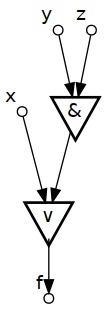
\includegraphics[height=150px]{scheme1.png}
\end{center}

Покажем минимальность этой схемы. Функция \(f(\widetilde{x}_3)\) существенно зависит от всех
своих переменных, поэтому по утверждению 16.1 \(L^C(f) \geq 3 - 1 = 2\).

Построим ДНФ для функции (2):
\begin{equation}
f(\widetilde{x}_3) = \overline{x}\overline{y}\overline{z}\vee x\overline{y}\overline{z}\vee
x\overline{y}z\vee xyz = \overline{y}\overline{z}\vee xz = \overline{y\vee z}\vee xz
\end{equation}
\clearpage

Соответствующая СФЭ имеет вид:
\begin{center}
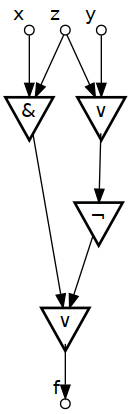
\includegraphics[height=200px]{scheme2.png}
\end{center}

Покажем минимальность этой схемы, т. е. что \(L^C(f) \geq 4\). Для этого заметим, что
\(f|_{x = 0} = \overline{y}\overline{z} \not\equiv const, f|_{x = 1} = \overline{(\overline{y}z)} \not\equiv const\).
Отсюда и из утверждения 16.3 следует, что \(L^C(f) \geq \min\{L^C(f|_{x = 0}), L^C(f|_{x = 1})\} + 2\).

Перебрав все элементы базиса, можно понять, что одного элемента не хватит ни для реализации
\(f|_{x = 0}\), ни для реализации \(f|_{x = 1}\). Таким образом, \(L^C(f) \geq 4\), что и
требовалось доказать.

Построим формулу для функции \(f\):
\begin{multline}
f(\widetilde{x}_3) = \overline{x}\overline{y}z\vee\overline{x}y\overline{z}\vee
x\overline{y}\overline{z}\vee xyz = \overline{x}(\overline{y}z\vee y\overline{z})\vee
x(\overline{y}\overline{z}\vee yz) = \overline{x}(\overline{\overline{y \vee z}\vee yz})\vee x(\overline{y\vee z}\vee yz) = \\
= \overline{x \vee \overline{y \vee z} \vee yz} \vee x(\overline{y \vee z}\vee yz)
\end{multline}

Получаем СФЭ:
\begin{center}
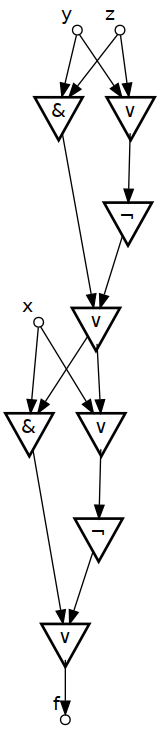
\includegraphics[height=300px]{scheme3.png}
\end{center}
\subsection{Задача 2.4(2)}
\label{sec:org57c3e2a}
Построить контактную схему сложности, не превышающей \(l\), реализующую функцию \(f\):
\begin{equation}
f(\widetilde{x}_3) = x_1\overline{x}_2 \oplus \overline{x}_2x_3 \oplus x_3x_1 \oplus 1, l = 5
\end{equation}
\subsubsection{Решение}
\label{sec:org82ecaf5}
Преобразуем \(f\) к удобному виду:
\begin{multline}
f(\widetilde{x}_3) = \overline{x}_1f|_{x_1 = 0}\vee x_1f|_{x_1 = 1} = \overline{x}_1(x_2\vee\overline{x}_3)\vee
x_1(\overline{x}_2\oplus \overline{x}_2x_3\oplus x_3\oplus1) = \overline{x}_1(x_2\vee\overline{x}_3)\vee x_1(\overline{x}_2\overline{x}_3\oplus\overline{x}_3) =\\
= \overline{x}_1x_2\vee\overline{x}_1\overline{x}_3\vee x_1x_2\overline{x_3} =
\overline{x}_1x_2\vee\overline{x}_1\overline{x}_3\vee x_2\overline{x_3}\vee x_1x_2\overline{x_3} =
\overline{x}_1(x_2\vee\overline{x}_3)\vee x_2\overline{x}_3
\end{multline}
Получаем КС:
\begin{center}
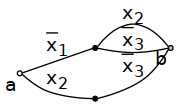
\includegraphics[height=100px]{scheme4.png}
\end{center}
\section{Домашняя работа 6}
\label{sec:orgedc555a}
\subsection{Задача 2.13(2, 6)}
\label{sec:orgcf79692}
С использованием метода каскадов построить контактную схему для функции \(f\):
\zall
\begin{equation}
f(\widetilde{x}^3) = x_1x_2 \vee x_2x_3 \vee x_3x_1
\end{equation}
\begin{equation}
f(\widetilde{x}^3) = (0110 1101)
\end{equation}
\subsubsection{Решение}
\label{sec:org534b23c}
Построим разложение Шеннона функции \(f\):
\begin{equation*}
\begin{cases}
f = x_1(x_2 \vee x_3 \vee x_2x_3) \vee \overline{x}_1x_2x_3 = \overline{x}_1f_0\vee x_1f_1,
f_0 = x_2x_3, f_1 = x_2\vee x_3, \widehat{G}_1 = G_1;
\end{cases}
\end{equation*}
\begin{equation*}
\begin{cases}
f_0 = x_2f_{01}\vee\overline{x}_2f_{00}, f_{00} = 0, f_{01} = x_3, \widehat{G}_2 = G_2 \\
f_1 = x_2f_{11}\vee\overline{x}_2f_{10}, f_{10} = x_3, f_{11} = 1;
\end{cases}
\end{equation*}
\begin{equation*}
\begin{cases}
f_{01} = x_3f_{011}\vee\overline{x}_3f_{010}, f_{011} = 1, f_{010} = 0, \widehat{G}_3 = G_3 \backslash \{f_{00}, f_{11}\} \\
f_{10} = x_3f_{101}\vee\overline{x}_3f_{100}, f_{101} = 1, f_{100} = 0;
\end{cases}
\end{equation*}
Тогда $G_4 = \widehat{G}_4 = \{f_{011}, f_{010}, f_{101}, f_{100}\} \cup \{G_3 \backslash \widehat{G}_3\} = \{0, 1\}$.
\pagebreak

Последовательно строим схему, начиная с $\widehat{G}_4$:
\begin{figure}[H]
\centering
\begin{tikzpicture}[>=latex']
\tikzstyle{pole} = [draw, shape=circle, inner sep=0pt, minimum size=1.5mm]
\tikzstyle{inner} = [draw, shape=circle, inner sep=0pt, minimum size=1.5mm, fill=black]
\begin{scope}
    \node[pole, label={0}] (0) {};
    \node[pole, label={1}] (1) [below=3cm of 0] {};
\end{scope}
\begin{scope}[xshift=2cm]
    \node[pole, label={0}, label={below:$f_{010}$}] (0) {};
    \node[pole, label={1}, label={below:$f_{011}$}] (1) [below=3cm of 0] {};
    \node[inner, color=blue, label={[blue]:$f_{01}$}] (2) [below right=1.5cm and 2cm of 0] {};
    \draw[color=blue] (0) -- (2) node[color=blue, midway, above] {$\overline{x}_3$};
    \draw[color=blue] (1) -- (2) node[color=blue, midway, above] {$x_3$};
\end{scope}
\begin{scope}[xshift=6cm]
    \node[pole, label={below:0}, label={$f_{010} = f_{00}$}] (0) {};
    \node[pole, label={1}, label={below:$f_{011} = f_{11}$}] (1) [below=3cm of 0] {};
    \node[inner, label={$f_{01}$}] (2) [below right=1.5cm and 2cm of 0] {};
    \node[inner, label={[blue]:$f_0$}] (3) [color=blue, below right=0.5cm and 3cm of 0] {};
    \node[inner, label={[blue]:$f_1$}] (4) [color=blue, below right=2.5cm and 3cm of 0] {};
    \draw (0) -- (2) node[midway, above] {$\overline{x}_3$};
    \draw (1) -- (2) node[midway, above] {$x_3$};
    \draw[color=blue] (0) -- (3) node[color=blue, midway, above] {$\overline{x}_2$};
    \draw[color=blue] (2) -- (3) node[color=blue, midway, above] {$x_2$};
    \draw[color=blue] (2) -- (4) node[color=blue, midway, above] {$\overline{x}_2$};
    \draw[color=blue] (1) -- (4) node[color=blue, midway, above] {$x_2$};
\end{scope}
\begin{scope}[xshift=11cm]
    \node[pole, label={below:0}, label={$f_{010} = f_{00}$}] (0) {};
    \node[pole, label={1}, label={below:$f_{011} = f_{11}$}] (1) [below=3cm of 0] {};
    \node[inner, label={$f_{01}$}] (2) [below right=1.5cm and 2cm of 0] {};
    \node[inner, label={$f_0$}] (3) [below right=0.5cm and 3cm of 0] {};
    \node[inner, label={$f_1$}] (4) [below right=2.5cm and 3cm of 0] {};
    \node[pole, label={[blue]:$f$}] (5) [color=blue, below right=1.5cm and 4cm of 0] {};
    \draw (0) -- (2) node[midway, above] {$\overline{x}_3$};
    \draw (1) -- (2) node[midway, above] {$x_3$};
    \draw (0) -- (3) node[midway, above] {$\overline{x}_2$};
    \draw (2) -- (3) node[midway, above] {$x_2$};
    \draw (2) -- (4) node[midway, above] {$\overline{x}_2$};
    \draw (1) -- (4) node[midway, above] {$x_2$};
    \draw[color=blue] (3) -- (5) node[color=blue, midway, above] {$\overline{x}_1$};
    \draw[color=blue] (4) -- (5) node[color=blue, midway, above] {$x_1$};
\end{scope}
\end{tikzpicture}
\end{figure}
Получили полную каскадную КС для функции (1). Функция $f$ реализуется подсхемой этой схемы,
проходящей между полюсами $1$ и $f$:
\begin{figure}[h]
\centering
\begin{tikzpicture}[>=latex']
\tikzstyle{pole} = [draw, shape=circle, inner sep=0pt, minimum size=1.5mm]
\tikzstyle{inner} = [draw, shape=circle, inner sep=0pt, minimum size=1.5mm, fill=black]
\node[pole, color=white] (0) {};
\node[pole, label={1}] (1) [below=3cm of 0] {};
\node[inner] (2) [below right=1.5cm and 2cm of 0] {};
\node[inner] (3) [below right=0.5cm and 3cm of 0] {};
\node[inner] (4) [below right=2.5cm and 3cm of 0] {};
\node[pole, label={$f$}] (5) [below right=1.5cm and 4cm of 0] {};
\draw (1) -- (2) node[midway, above] {$x_3$};
\draw (2) -- (3) node[midway, above] {$x_2$};
\draw (2) -- (4) node[midway, above] {$\overline{x}_2$};
\draw (1) -- (4) node[midway, above] {$x_2$};
\draw (3) -- (5) node[midway, above] {$\overline{x}_1$};
\draw (4) -- (5) node[midway, above] {$x_1$};
\end{tikzpicture}
\end{figure}


Построим теперь разложение для второй функции:
\begin{equation*}
\begin{cases}
f = \overline{x}_1f_0\vee x_1f_1, f_0 = (0110), f_1 = (1101), \widehat{G}_1 = G_1;
\end{cases}
\end{equation*}
\begin{equation*}
\begin{cases}
f_0 = \overline{x}_2f_{00}\vee x_2f_{01}, f_{00} = (01) = x_3, f_{01} = (10) = \overline{x}_3, \widehat{G}_2 = G_2 \\
f_1 = \overline{x}_2f_{10}\vee x_2f_{11}, f_{10} = (11) = 1, f_{11} = (01) = x_3;
\end{cases}
\end{equation*}
\begin{equation*}
\begin{cases}
f_{00} = \overline{x}_3f_{000}\vee x_3f_{001}, f_{000} = 0, f_{001} = 1, \widehat{G}_3 = G_3 \backslash \{f_{10}\} \\
f_{01} = \overline{x}_3f_{010}\vee x_3f_{011}, f_{010} = 1, f_{011} = 0, \\
f_{11} = \overline{x}_3f_{110}\vee x_3f_{111}, f_{110} = 0, f_{111} = 1;
\end{cases}
\end{equation*}
\begin{equation*}
G_4 = \widehat{G}_4 = \{f_{000}, f_{001}, f_{010}, f_{011}, f_{110}, f_{111}\} \cup G_3 \backslash \widetilde{G}_3 = \{0, 1\}
\end{equation*}
Построим полную КС, начиная с $\widetilde{G}_4$:
\begin{figure}[H]
\centering
\begin{tikzpicture}
\tikzstyle{pole} = [draw, shape=circle, inner sep=0mm, minimum size=1.5mm]
\tikzstyle{inner} = [draw, shape=circle, inner sep=0mm, minimum size=1.5mm, fill=black]

\begin{scope}
    \node[pole, label={0}] (0) {};
    \node[pole, label={1}] (1) [below = 3cm of 0] {};
\end{scope}

\begin{scope}[xshift=2cm]
    \node[pole, label={0}] (0) {};
    \node[pole, label={1}, label={below:$f_{010} = f_{10}$}] (1) [below = 3cm of 0] {};
    \node[inner, color=blue, label={[blue]:$f_{00}$}] (2) [below right = 0.5cm and 1.5cm of 0] {};
    \node[inner, color=blue, label={[blue]:$f_{01}$}] (3) [above right = 0.5cm and 1.5cm of 1] {};

    \draw[color=blue] (0) -- (2) node[color=blue, midway, above] {$\overline{x}_3$};
    \draw[color=blue] (1) -- (2) node[color=blue, midway, above] {$x_3$};
    \draw[color=blue] (0) -- (3) node[color=blue, midway, above] {$x_3$};
    \draw[color=blue] (1) -- (3) node[color=blue, midway, above] {$\overline{x}_3$};
\end{scope}

\begin{scope}[xshift=5cm]
    \node[pole, label={0}] (0) {};
    \node[pole, label={1}, label={below:$f_{010} = f_{10}$}] (1) [below = 3cm of 0] {};
    \node[inner, label={$f_{00}$}] (2) [right = 1.5cm of 0] {};
    \node[inner, label={below:$f_{01}$}] (3) [right = 1.5cm of 1] {};
    \node[inner, color=blue, label={[blue]:$f_0$}] (4) [below right = 0.5cm and 1.5cm of 2] {};
    \node[inner, color=blue, label={[blue]:$f_1$}] (5) [above right = 0.5cm and 1.5cm of 3] {};

    \draw (0) -- (2) node[midway, above] {$\overline{x}_3$};
    \draw (1) -- (2) node[midway, above] {$x_3$};
    \draw (0) -- (3) node[midway, above] {$x_3$};
    \draw (1) -- (3) node[midway, above] {$\overline{x}_3$};
    \draw[color=blue] (2) -- (4) node[midway, above, color=blue] {$\overline{x}_2$};
    \draw[color=blue] (3) -- (4) node[midway, above, color=blue] {$x_2$};
    \draw[color=blue] (1) -- (5) node[midway, above, color=blue] {$\overline{x}_2$};
    \draw[color=blue] (2) -- (5) node[midway, above, color=blue] {$x_2$};
\end{scope}

\begin{scope}[xshift=10cm]
    \node[pole, label={0}] (0) {};
    \node[pole, label={1}, label={below:$f_{010} = f_{10}$}] (1) [below = 3cm of 0] {};
    \node[inner, label={$f_{00}$}] (2) [right = 1.5cm of 0] {};
    \node[inner, label={below:$f_{01}$}] (3) [right = 1.5cm of 1] {};
    \node[inner, label={$f_0$}] (4) [below right = 0.5cm and 1.5cm of 2] {};
    \node[inner, label={$f_1$}] (5) [above right = 0.5cm and 1.5cm of 3] {};
    \node[pole, label={[blue]:$f$}, color=blue] (6) [below right = 0.75cm and 1cm of 4] {};

    \draw (0) -- (2) node[midway, above] {$\overline{x}_3$};
    \draw (1) -- (2) node[midway, above] {$x_3$};
    \draw (0) -- (3) node[midway, above] {$x_3$};
    \draw (1) -- (3) node[midway, above] {$\overline{x}_3$};
    \draw (2) -- (4) node[midway, above] {$\overline{x}_2$};
    \draw (3) -- (4) node[midway, above] {$x_2$};
    \draw (1) -- (5) node[midway, above] {$\overline{x}_2$};
    \draw (2) -- (5) node[midway, above] {$x_2$};
    \draw[color=blue] (4) -- (6) node[midway, above, color=blue] {$\overline{x}_1$};
    \draw[color=blue] (5) -- (6) node[midway, above, color=blue] {$x_1$};
\end{scope}
\end{tikzpicture}
\end{figure}
КС, реализующая функцию $f$:
\begin{figure}[H]
\centering
\begin{tikzpicture}[>=latex']
\tikzstyle{pole} = [draw, shape=circle, inner sep=0pt, minimum size=1.5mm]
\tikzstyle{inner} = [draw, shape=circle, inner sep=0pt, minimum size=1.5mm, fill=black]

    \node[pole, color=white, label={}] (0) {};
    \node[pole, label={1}, label={below:$f_{010} = f_{10}$}] (1) [below = 3cm of 0] {};
    \node[inner, label={$f_{00}$}] (2) [right = 1.5cm of 0] {};
    \node[inner, label={below:$f_{01}$}] (3) [right = 1.5cm of 1] {};
    \node[inner, label={$f_0$}] (4) [below right = 0.5cm and 1.5cm of 2] {};
    \node[inner, label={$f_1$}] (5) [above right = 0.5cm and 1.5cm of 3] {};
    \node[pole, label={$f$}] (6) [below right = 0.75cm and 1cm of 4] {};

    \draw (1) -- (2) node[midway, above] {$x_3$};
    \draw (1) -- (3) node[midway, above] {$\overline{x}_3$};
    \draw (2) -- (4) node[midway, above] {$\overline{x}_2$};
    \draw (3) -- (4) node[midway, above] {$x_2$};
    \draw (1) -- (5) node[midway, above] {$\overline{x}_2$};
    \draw (2) -- (5) node[midway, above] {$x_2$};
    \draw (4) -- (6) node[midway, above] {$\overline{x}_1$};
    \draw (5) -- (6) node[midway, above] {$x_1$};
\end{tikzpicture}
\end{figure}
\subsection{Задача 2.14(2)}
\label{sec:org6850848}
С использованием метода каскадов построить контактную схему для системы функций \(\Phi\):
\begin{equation}
\Phi = \{x_2 \oplus x_3, x_1 \oplus x_2 \oplus x_3, \overline{x}_2\}
\end{equation}
\subsubsection{Решение}
\label{sec:org9d608fd}
Строим разложение Шеннона для функций системы:
\begin{equation*}
\begin{cases}
f = x_2 \oplus x_3, \\
g = x_1 \oplus x_2 \oplus x_3, \\
h = \overline{x}_2;
\end{cases}
\end{equation*}
\begin{equation*}
\begin{cases}
g = \overline{x}_1g_0\vee x_1g_1, g_0 = x_2 \oplus x_3, g_1 = x_2 \oplus x_3 \oplus 1, \widehat{G}_1 = G_1 \backslash \{f, h\};
\end{cases}
\end{equation*}
\begin{equation*}
\begin{cases}
f = g_0 = \overline{x}_2f_0\vee x_2f_1, f_0 = x_3, f_1 = \overline{x}_3, \widehat{G}_2 = G_2, \\
g_1 = \overline{x}_2g_{10}\vee x_2g_{11}, g_{10} = \overline{x}_3, g_{11} = x_3, \\
h = \overline{x}_2h_0\vee x_2h_1, h_0 = 1, h_1 = 0;
\end{cases}
\end{equation*}
\begin{equation*}
\begin{cases}
f_0 = g_{11} = \overline{x}_3f_{00}\vee x_3f_{01}, f_{00} = 0, f_{01} = 1, \widehat{G}_3 = G_3 \backslash \{h_0, h_1\}, \\
f_1 = g_{10} = \overline{x}_3f_{10}\vee x_3f_{11}, f_{10} = 1, f_{10} = 0;
\end{cases}
\end{equation*}
\begin{equation*}
\widehat{G}_4 = G_4 = \{0, 1\}
\end{equation*}
\pagebreak

Строим полную каскадную КС:
\begin{figure}[H]
\centering
\begin{tikzpicture}[>=latex']
\tikzstyle{pole} = [draw, shape=circle, inner sep=0pt, minimum size=1.5mm]
\tikzstyle{inner} = [draw, shape=circle, inner sep=0pt, minimum size=1.5mm, fill=black]

\begin{scope}
    \begin{dot2tex}[dot, tikz, codeonly, options=-tmath]
    graph G {
        rankdir="LR";
        node [style="pole", label=""];
        1[xlabel="1"];
        0[xlabel="0"];
    }
    \end{dot2tex}
\end{scope}

\begin{scope}[xshift=3cm]
    \begin{dot2tex}[dot, tikz, codeonly, options=-s -tmath]
    graph G {
        rankdir="LR";
        node[style="pole", label=""];
        0[xlabel="0"];
        1[xlabel="1"];
        node[style="inner", color=blue];
        2[xlabel="g_{10}"];
        3[xlabel="g_{11}"];
        0 -- 2 [color=blue, label="x_3"];
        0 -- 3 [color=blue, texlbl="$\overline{x}_3$", label=" "];
        1 -- 2 [color=blue, texlbl="$\overline{x}_3$", label=" "];
        1 -- 3 [color=blue, label="x_3"];
    }
    \end{dot2tex}
\end{scope}

\begin{scope}[xshift=8cm]
    \begin{dot2tex}[dot, tikz, codeonly, options=-s -tmath]
    graph G {
        rankdir="LR";
        node[style="pole", label=""];
        0[xlabel="0"];
        1[xlabel="1"];
        node[style="inner"];
        2[xlabel="g_{10}"];
        3[xlabel="g_{11}"];
        4[xlabel="f", style="pole"];
        5[xlabel="g_1"];
        6[xlabel="h", style="pole"];
        0 -- 2 [label="x_3"];
        0 -- 3 [texlbl="$\overline{x}_3$", label=" "];
        1 -- 2 [texlbl="$\overline{x}_3$", label=" "];
        1 -- 3 [label="x_3"];
        2 -- 4 [color=blue, label="x_2"];
        3 -- 4 [color=blue, texlbl="$\overline{x}_2$" label=" "];
        2 -- 5 [color=blue, texlbl="$\overline{x}_2$" label=" "];
        3 -- 5 [color=blue, label="x_2"];
        0 -- 6 [color=blue, label="x_2"];
        1 -- 6 [color=blue, texlbl="$\overline{x}_2$" label=" "];
    }
    \end{dot2tex}
\end{scope}
\end{tikzpicture}
\end{figure}
\begin{figure}[H]
\centering
\begin{tikzpicture}[>=latex']
\tikzstyle{pole} = [draw, shape=circle, inner sep=0pt, minimum size=1.5mm]
\tikzstyle{inner} = [draw, shape=circle, inner sep=0pt, minimum size=1.5mm, fill=black]

\begin{dot2tex}[dot, tikz, codeonly, options=-s -tmath]
graph G {
    rankdir="LR";
    node[style="pole", label=""];
    0[xlabel="0"];
    1[xlabel="1"];
    node[style="inner"];
    2[xlabel="g_{10}"];
    3[xlabel="g_{11}"];
    4[xlabel="f", style="pole"];
    5[xlabel="g_1"];
    6[xlabel="h", style="pole"];
    7[xlabel="g", style="pole"];
    0 -- 2 [label="x_3"];
    0 -- 3 [texlbl="$\overline{x}_3$", label=" "];
    1 -- 2 [texlbl="$\overline{x}_3$", label=" "];
    1 -- 3 [label="x_3"];
    2 -- 4 [label="x_2"];
    3 -- 4 [texlbl="$\overline{x}_2$", label=" "];
    2 -- 5 [texlbl="$\overline{x}_2$", label=" "];
    3 -- 5 [label="x_2"];
    0 -- 6 [label="x_2"];
    1 -- 6 [texlbl="$\overline{x}_2$", label=" "];
    4 -- 7 [color=blue, texlbl="$\overline{x}_1$", label=" "];
    5 -- 7 [color=blue, label="x_1"];
}
\end{dot2tex}
\end{tikzpicture}
\end{figure}

КС, реализующая систему функций:
\begin{figure}[H]
\centering
\begin{tikzpicture}[>=latex']
\tikzstyle{pole} = [draw, shape=circle, inner sep=0pt, minimum size=1.5mm]
\tikzstyle{inner} = [draw, shape=circle, inner sep=0pt, minimum size=1.5mm, fill=black]

\begin{dot2tex}[dot, tikz, codeonly, options=-s -tmath]
graph G {
    rankdir="LR";
    node[style="pole", label=""];
    1[xlabel="1"];
    node[style="inner"];
    2[xlabel="g_{10}"];
    3[xlabel="g_{11}"];
    4[xlabel="f", style="pole"];
    5[xlabel="g_1"];
    6[xlabel="h", style="pole"];
    7[xlabel="g", style="pole"];
    1 -- 2 [texlbl="$\overline{x}_3$", label=" "];
    1 -- 3 [label="x_3"];
    2 -- 4 [label="x_2"];
    3 -- 4 [texlbl="$\overline{x}_2$", label=" "];
    2 -- 5 [texlbl="$\overline{x}_2$", label=" "];
    3 -- 5 [label="x_2"];
    1 -- 6 [texlbl="$\overline{x}_2$", label=" "];
    4 -- 7 [color=blue, texlbl="$\overline{x}_1$", label=" "];
    5 -- 7 [color=blue, label="x_1"];
}
\end{dot2tex}
\end{tikzpicture}
\end{figure}
\subsection{Задача 2.14(6, КС и СФЭ)}
\label{sec:org37ffbe6}
С использованием метода каскадов построить КС и СФЭ для системы функций \(\Phi\):
\begin{equation}
\Phi = \{f_1 = x_1\overline{x}_2x_3\vee\overline{x}_1x_2\overline{x}_3, f_2 = x_1\overline{x}_3\vee\overline{x}_2\}
\end{equation}
\subsubsection{Решение}
\label{sec:org7c23dd5}
Строим разложение Шеннона:
\begin{equation*}
\begin{cases}
f_1 = \overline{x}_1f_{10}\vee x_1f_{11}, f_{10} = x_2\overline{x}_3, f_{11} = \overline{x}_2x_3, \widehat{G}_1 = G_1, \\
f_2 = \overline{x}_1f_{20}\vee x_2f_{21}, f_{20} = \overline{x}_3, f_{21} = \overline{x}_2;
\end{cases}
\end{equation*}
\begin{equation*}
\begin{cases}
f_{10} = \overline{x}_2f_{100}\vee x_2f_{101}, f_{100} = 0, f_{101} = \overline{x}_3, \widehat{G}_2 = G_2 \backslash \{f_{20}\}, \\
f_{11} = \overline{x}_2f_{110}\vee x_2f_{111}, f_{110} = x_3, f_{111} = 0, \\
f_{21} = \overline{x}_2f_{210}\vee x_2f_{211}, f_{210} = 1, f_{211} = 0;
\end{cases}
\end{equation*}
\begin{equation*}
G_3 = \{1, x_3\}, \widehat{G}_3 = \{x_3\}
\end{equation*}

Получаем КС:
\begin{figure}[H]
\centering
\begin{tikzpicture}[>=latex']
\tikzstyle{pole} = [draw, shape=circle, inner sep=0pt, minimum size=1.5mm]
\tikzstyle{inner} = [draw, shape=circle, inner sep=0pt, minimum size=1.5mm, fill=black]

\begin{dot2tex}[dot, tikz, codeonly, options=-s -tmath]
graph {
    rankdir=LR
    node[style=pole, label=" "];
    1[xlabel="1"];
    f1[xlabel="f_1"];
    f2[xlabel="f_2"];
    node[style=inner];
    f110; f20; f10; f11; f21;
    1 -- f110 [label="x_3"];
    1 -- f20 [label=" " texlbl="$\overline{x}_3$"];
    1 -- f21 [label=" " texlbl="$\overline{x}_2$"];
    f110 -- f11 [label=" " texlbl="$\overline{x}_2$"];
    f20 -- f10 [label="x_2"];
    f10 -- f1 [label=" " texlbl="$\overline{x}_1$"];
    f11 -- f1 [label="x_1"];
    f20 -- f2 [label=" " texlbl="$\overline{x}_2$"];
    f21 -- f2 [label="x_2"];
}
\end{dot2tex}
\end{tikzpicture}
\end{figure}
Соответствующая СФЭ:
\begin{figure}[H]
\centering
\begin{tikzpicture}[>=latex', scale=0.5]
\tikzstyle{pole} = [draw, shape=circle, inner sep=0pt, minimum size=1.5mm]

\begin{dot2tex}[dot, tikz, codeonly, options=-tmath]
digraph {
    node [style=pole, label=" "];
    x1[xlabel="x_1"]; x2[xlabel="x_2"]; x3[xlabel="x_3"];
    f1[xlabel="f_1"]; f2[xlabel="f_2"];
    node [shape=triangle, style="thick, rotate=180", lblstyle="rotate=180"];
    f20[label="\neg"]; f21[label="\neg"];
    f10[label="\&"]; f11[label="\&"];
    nx1[label="\neg"];
    v1[label="\&"]; v2[label="\&"]; v3[label="\vee"];
    v4[label="\&"]; v5[label="\&"]; v6[label="\vee"];
    x3 -> f20; x2 -> f21; x2 -> f10;
    f20 -> f10; x3 -> f11; f21 -> f11;
    x1 -> nx1; nx1 -> v1; f10 -> v1;
    x1 -> v2; f11 -> v2;
    v1 -> v3; v2 -> v3; v3 -> f1;
    nx1 -> v4; f20 -> v4;
    x1 -> v5; f21 -> v5;
    v4 -> v6; v5 -> v6; v6 -> f2
}
\end{dot2tex}
\end{tikzpicture}
\end{figure}
\subsection{Задача}
\label{sec:orga65909a}
С помощью метода Шеннона, разлагая ФАЛ \(f(x_1, x_2, x_3)\), заданную столбцом значений
\((0100 1011)\), по переменным \(x_1\) и \(x_2\), построить КС, реализующую эту функцию.
\subsubsection{Решение}
\label{sec:org50af64e}
Разложим функцию $f$ по первым двум переменным:
\begin{equation}
\begin{cases}
f(0, 0, x_3) = x_3, \\
f(0, 1, x_3) = 0, \\
f(1, 0, x_3) = \overline{x}_3, \\
f(1, 1, x_3) = 1.
\end{cases}
\end{equation}
Строим контактное дерево и универсальный многополюсник от переменной $x_3$:
\begin{figure}[H]
\centering
\begin{tikzpicture}[>=latex']
\tikzstyle{pole} = [draw, shape=circle, inner sep=0pt, minimum size=1.5mm]
\tikzstyle{inner} = [draw, shape=circle, inner sep=0pt, minimum size=1.5mm, fill=black]

\begin{scope}
\begin{dot2tex}[dot, tikz, codeonly, options=-s -tmath]
graph {
    rankdir=LR;
    node[style=pole, label=""]; 1[xlabel="1"];
    node[style=inner];
    1 -- v1  [label=" ", texlbl="$x_1$"];
    1 -- v2  [label=" ", texlbl="$\overline{x}_1$"];
    v1 -- v3 [label=" ", texlbl="$x_2$"];
    v1 -- v4 [label=" ", texlbl="$\overline{x}_2$"];
    v2 -- v5 [label=" ", texlbl="$x_2$"];
    v2 -- v6 [label=" ", texlbl="$\overline{x}_2$"];
}
\end{dot2tex}
\end{scope}

\begin{scope}[xshift=10cm]
\begin{dot2tex}[dot, tikz, codeonly, options=-s -tmath]
graph {
    rankdir=LR;
    node[style=pole, label=""];
    1 -- 3 [label=" ", texlbl="$x_3$"];
    2 -- 3 [label=" ", texlbl="$\overline{x}_3$"];
}
\end{dot2tex}
\end{scope}
\end{tikzpicture}
\end{figure}
Соединяем выходы контактного дерева c входами многополюсника:
\begin{figure}[H]
\centering
\begin{tikzpicture}[>=latex']
\tikzstyle{pole} = [draw, shape=circle, inner sep=0pt, minimum size=1.5mm]
\tikzstyle{inner} = [draw, shape=circle, inner sep=0pt, minimum size=1.5mm, fill=black]

\begin{dot2tex}[dot, tikz, codeonly, options=-tmath]
graph {
    rankdir=LR;
    node[style=pole, label=""]; 1[xlabel="1"]; f[xlabel="f"];
    node[style=inner];
    1 -- v1  [label=" ", texlbl="$x_1$"];
    1 -- v2  [label=" ", texlbl="$\overline{x}_1$"];
    v1 -- f  [label=" ", texlbl="$x_2$"];
    v1 -- v4 [label=" ", texlbl="$\overline{x}_2$"];
    v2 -- v6 [label=" ", texlbl="$\overline{x}_2$"];
    v4 -- f  [label=" ", texlbl="$\overline{x}_3$"];
    v6 -- f  [label=" ", texlbl="$x_3$"];
}
\end{dot2tex}
\end{tikzpicture}
\end{figure}
\section{Домашняя работа 7}
\label{sec:orgeccc567}
\subsection{Задача 5.1(5, 6)}
\label{sec:orgb1dcdfd}
Построить все тупиковые диагностические тесты для матрицы
\begin{equation}
M = \begin{pmatrix}
1 & 1 & 1 & 0 & 0 \\
0 & 1 & 1 & 1 & 0 \\
0 & 0 & 1 & 1 & 1 \\
1 & 0 & 0 & 1 & 1 \\
1 & 1 & 0 & 0 & 1
\end{pmatrix}
\end{equation}
Построить все тупиковые проверяющие тесты для матрицы
\begin{equation}
M = \begin{pmatrix}
1 & 0 & 1 & 0 & 0 & 1 & 0 \\
1 & 0 & 0 & 1 & 0 & 0 & 1 \\
0 & 1 & 0 & 1 & 0 & 1 & 0 \\
0 & 0 & 1 & 0 & 1 & 1 & 0 \\
0 & 1 & 0 & 0 & 1 & 0 & 1
\end{pmatrix}
\end{equation}
\subsubsection{Решение}
\label{sec:orgc43c366}
Цель контроля для задачи диагностики матрицы \(M\) имеет вид \(\mathcal{N} = \{(i, j) | 1 \leq i < j \leq 5\}\).
Сопоставим i-й строке матрицы \(M\) переменную \(y_i\) и построим матрицу \(\mathcal{M}\),
состоящую из покоординатных сумм по модулю 2 столбцов входящих, в \(\mathcal{N}\):
\begin{equation*}
\mathcal{M} = \begin{pmatrix}
0 & 0 & 1 & 1 & 0 & 1 & 1 & 1 & 1 & 0 \\
1 & 1 & 1 & 0 & 0 & 0 & 1 & 0 & 1 & 1 \\
0 & 1 & 1 & 1 & 1 & 1 & 1 & 0 & 0 & 0 \\
1 & 1 & 0 & 0 & 0 & 1 & 1 & 1 & 1 & 0 \\
0 & 1 & 1 & 0 & 1 & 1 & 0 & 0 & 1 & 1
\end{pmatrix}
\end{equation*}
Построим КНФ функции диагностического теста для матрицы \(M\):
\begin{multline*}
F(y_1, y_2, y_3, y_4) = (y_2\lor y_4)(y_2\lor y_3\lor y_4\lor y_5)(y_1\lor y_2\lor y_3\lor y_5)
(y_1\lor y_3)(y_3\lor y_5)(y_1\lor y_3\lor y_4\lor y_5)\\
(y_1\lor y_2\lor y_3\lor y_4)(y_1\lor y_4)(y_1\lor y_2\lor y_4\lor y_5)(y_2\lor y_5) =
(y_1\lor y_3)(y_1\lor y_4)(y_2\lor y_4)(y_2\lor y_5)(y_3\lor y_5) = \\
= (y_1\lor y_3y_4)(y_2\lor y_4y_5)(y_3\lor y_5) = (y_1\lor y_3y_5)(y_2y_3\lor y_3y_4y_5\lor y_4y_5\lor y_2y_5) =
y_1y_2y_3\lor y_1y_4y_5\lor y_1y_2y_5\lor y_2y_3y_5\lor y_3y_4y_5
\end{multline*}
Каждое слагамое полученной сокращённой ДНФ отвечает одному диагностическому тесту. Таким образом,
все тупиковые диагностические тесты матрицы \(M\) соответствуют следующим множествам номеров
строк \(M\): \(\{1, 2, 3\}, \{1, 2, 5\}, \{1, 4, 5\}, \{2, 3, 5\}, \{3, 4, 5\}\).

Цель контроля для проверки следующей матрицы \(M\) имеет вид \(\mathcal{N} = \{(1, i) | 1 \leq i \leq 7\}\).
Сопоставим i-й строке матрицы \(M\) переменную \(y_i\) и построим матрицу \(\mathcal{M}\), состоящую
из покоординатных сумм по модулю 2 столбцов, входящих в \(\mathcal{N}\):
\begin{equation*}
\mathcal{M} = \begin{pmatrix}
1 & 0 & 1 & 1 & 0 & 1 \\
1 & 1 & 0 & 1 & 1 & 0 \\
1 & 0 & 1 & 0 & 1 & 0 \\
0 & 1 & 0 & 1 & 1 & 0 \\
1 & 0 & 0 & 1 & 0 & 1
\end{pmatrix}
\end{equation*}
Функция проверяющего теста для матрицы \(M\):
\begin{multline*}
F(y_1, y_2, y_3, y_4, y_5) = (y_1\lor y_2\lor y_3\lor y_5)(y_2\lor y_4)(y_1\lor y_3)
(y_1\lor y_2\lor y_4\lor y_5)(y_2\lor y_3\lor y_4)(y_1\lor y_5) = \\
= (y_1\lor y_3)(y_1\lor y_5)(y_2\lor y_4) = (y_1\lor y_3y_5)(y_2\lor y_4) =
y_1y_2\lor y_2y_3y_5\lor y_1y_4\lor y_3y_4y_5
\end{multline*}
Каждое слагаемое полученной сокращённой ДНФ отвечает одному проверяющему тесту, что означает,
что все тупиковые проверяющие тесты матрицы \(M\) соответствуют множествам наборов строк \(M\):
\(\{1, 2\}, \{1, 4\}, \{2, 3, 5\}, \{3, 4, 5\}\).
\subsection{Задача 6.3}
\label{sec:org9245f3b}
Построить все тупиковые
\begin{enumerate}
\item проверяющие
\item диагностические
\end{enumerate}
тесты для КС:
\begin{figure}[H]
\centering
\begin{tikzpicture}[>=latex']
\tikzstyle{pole} = [draw, shape=circle, inner sep=0pt, minimum size=1.5mm]
\tikzstyle{inner} = [draw, shape=circle, inner sep=0pt, minimum size=1.5mm, fill=black]

\begin{dot2tex}[dot, tikz, codeonly, options=-tmath -s]
graph G {
    rankdir=LR;
    node[style=pole, label=""] a[xlabel="a"]; b[xlabel="b"];
    node[style=inner];
    a  -- v1 [label=" ", texlbl="$x$"];
    a  -- v2 [label=" ", texlbl="$\overline{x}$"];
    v1 -- v3 [label=" ", texlbl="$y$"];
    v1 -- v4 [label=" ", texlbl="$\overline{y}$"];
    v2 -- v3 [label=" ", texlbl="$\overline{y}$"];
    v2 -- v4 [label=" ", texlbl="$y$"];
    v3 -- b  [label=" ", texlbl="$\overline{z}$"];
    v4 -- b  [label=" ", texlbl="$z$"];
}
\end{dot2tex}
\end{tikzpicture}
\end{figure}
и источника, допускающего обрыв одного контакта переменных \(x\), \(z\).
\subsubsection{Решение}
\label{sec:org42005fc}
Вычислим таблицу контроля для заданной схемы и источника неисправностей:
\begin{center}
\begin{tabular}{rrrrrrl}
\hline
\(xyz\) & \(f\) & \(f_{x}\) & \(f_{\overline{x}}\) & \(f_z\) & \(f_{\overline{z}}\) & \\
\hline
000 & 1 & 1 & 0 & 1 & 0 & \(y_1\)\\
001 & 0 & 0 & 0 & 0 & 0 & \(y_2\)\\
010 & 0 & 0 & 0 & 0 & 0 & \(y'_2\)\\
011 & 1 & 1 & 0 & 0 & 1 & \(y_3\)\\
100 & 0 & 0 & 0 & 0 & 0 & \(y''_2\)\\
101 & 1 & 0 & 1 & 1 & 0 & \(y_4\)\\
110 & 1 & 0 & 1 & 1 & 0 & \(y'_4\)\\
111 & 0 & 0 & 0 & 0 & 0 & \(y_5\)\\
\hline
\end{tabular}
\end{center}
Отсюда получаем матрицу контроля \(M\):
\begin{equation*}
M = \begin{pmatrix}
1 & 1 & 0 & 1 & 0 \\
0 & 0 & 0 & 0 & 0 \\
1 & 1 & 0 & 0 & 1 \\
1 & 0 & 1 & 1 & 0
\end{pmatrix}
\end{equation*}
\begin{enumerate}
\item Цель контроля для задачи диагностики \(\mathcal{N} = \{(i, j) | 1 \leq i < j \leq 5\}\).
\end{enumerate}
Соответствующая матрица \(\mathcal{M}\):
\begin{equation*}
\mathcal{M} = \begin{pmatrix}
0 & 1 & 0 & 1 & 1 & 0 & 1 & 1 & 0 & 1 \\
0 & 0 & 0 & 0 & 0 & 0 & 0 & 0 & 0 & 0 \\
0 & 1 & 1 & 0 & 1 & 1 & 0 & 0 & 1 & 1 \\
1 & 0 & 0 & 1 & 1 & 1 & 0 & 0 & 1 & 1
\end{pmatrix} = \begin{pmatrix}
0 & 1 & 0 & 1 & 1 & 0 & 1 \\
0 & 0 & 0 & 0 & 0 & 0 & 0 \\
0 & 1 & 1 & 0 & 1 & 1 & 0 \\
1 & 0 & 0 & 1 & 1 & 1 & 0
\end{pmatrix}
\end{equation*}
Функция покрытия:
\begin{equation*}
F(y_1, y_2, y_3, y_4) = y_4(y_1\lor y_3)y_3(y_1\lor y_4)(y_1\lor y_3\lor y_4)(y_3\lor y_4)y_1 =
y_1y_3y_4
\end{equation*}
Это даёт следующий набор тупиковых диагностических тестов:
$\{(000), (011), (101)\}, \{(000), (011), (110)\}$.
\begin{enumerate}
\item Цель контроля для задачи проверки \(\mathcal{N} = \{(1, i) | 1 < i \leq 5\}\).
\end{enumerate}
Соответствующая матрица \(\mathcal{M}\):
\begin{equation*}
\mathcal{M} = \begin{pmatrix}
0 & 1 & 0 & 1 \\
0 & 0 & 0 & 0 \\
0 & 1 & 1 & 0 \\
1 & 0 & 0 & 1
\end{pmatrix}
\end{equation*}
Функция покрытия:
\begin{equation*}
F(y_1, y_2, y_3, y_4) = y_4(y_1\lor y_3)y_3(y_1\lor y_4) = y_3y_4
\end{equation*}
Соответствующий набор тупиковых проверяющих тестов:
$\{(011), (101)\}, \{(011), (110)\}$.
\subsection{Задача 6.5}
\label{sec:org5426232}
Построить все тупиковые:
\begin{enumerate}
\item проверяющие
\item диагностические
\end{enumerate}
тесты для КС:
\begin{figure}[H]
\centering
\begin{tikzpicture}[>=latex']
\tikzstyle{pole} = [draw, shape=circle, inner sep=0pt, minimum size=1.5mm]
\tikzstyle{inner} = [draw, shape=circle, inner sep=0pt, minimum size=1.5mm, fill=black]

\begin{dot2tex}[dot, tikz, codeonly, options=-tmath -s]
graph G {
    rankdir=LR;
    node[style=pole, label=""] a[xlabel="a"]; b[xlabel="b"];
    node[style=inner];
    a  -- v1 [label=" ", texlbl="$\overline{z}$"];
    a  -- v2 [label=" ", texlbl="$x$"];
    v1 -- v2 [label=" ", texlbl="$\overline{x}$"];
    v1 -- v3 [label=" ", texlbl="$\overline{y}$"];
    v2 -- v3 [label=" ", texlbl="$z$"];
    v2 -- b  [label=" ", texlbl="$\overline{x}$"];
    v3 -- b  [label=" ", texlbl="$y$"];
}
\end{dot2tex}
\end{tikzpicture}
\end{figure}
с единичным источником неисправностей, допускающим обрыв контактов вида \(z, \overline{z}\), или
замыкание контакта вида \(y\).
\subsubsection{Решение}
\label{sec:orgdf9f446}
Вычислим таблицу контроля для заданной схемы и заданного источника неисправностей:
\begin{center}
\begin{tabular}{rrrrrrl}
\hline
\(xyz\) & \(f\) & \(f_{z}\) & \(f_{\overline{z}}\) & \(f_{z\overline{z}}\) & \(f_y\) & \\
\hline
000 & 1 & 1 & 0 & 0 & 1 & \(y_1\)\\
001 & 0 & 0 & 0 & 0 & 0 & \(y_2\)\\
010 & 1 & 1 & 0 & 0 & 1 & \(y'_1\)\\
011 & 0 & 0 & 0 & 0 & 0 & \(y'_2\)\\
100 & 0 & 0 & 0 & 0 & 1 & \(y_3\)\\
101 & 0 & 0 & 0 & 0 & 1 & \(y'_3\)\\
110 & 0 & 0 & 0 & 0 & 0 & \(y''_2\)\\
111 & 1 & 0 & 1 & 0 & 1 & \(y_4\)\\
\hline
\end{tabular}
\end{center}
Получаем матрицу контроля \(M\):
\begin{equation*}
M = \begin{pmatrix}
1 & 1 & 0 & 0 & 1 \\
0 & 0 & 0 & 0 & 0 \\
0 & 0 & 0 & 0 & 1 \\
1 & 0 & 1 & 0 & 1
\end{pmatrix}
\end{equation*}
\begin{enumerate}
\item Цель контроля для задачи диагностики -- множество \(\mathcal{N} = \{(i, j) | 1 \leq i < j \leq 5\}\).
\end{enumerate}
Соответствующая матрица \(\mathcal{M}\):
\begin{equation*}
\mathcal{M} = \begin{pmatrix}
0 & 1 & 1 & 0 & 0 & 1 & 1 \\
0 & 0 & 0 & 0 & 0 & 0 & 0 \\
0 & 0 & 0 & 1 & 1 & 1 & 1 \\
1 & 0 & 1 & 0 & 1 & 0 & 1
\end{pmatrix}
\end{equation*}
Функция покрытия для этой матрицы:
\begin{equation*}
F(y_1, y_2, y_3, y_4) = y_4y_1(y_1\lor y_4)y_3(y_3\lor y_4)(y_1\lor y_3)(y_1\lor y_3\lor y_4) =
y_1y_3y_4
\end{equation*}
Что даёт следующий набор тупиковых диагностических тестов:
$$\{(000), (100), (111)\}, \{(010), (100), (111)\}, \{(000), (101), (111)\}, \{(010), (101), (111)\}$$
\begin{enumerate}
\item Цель контроля для задачи проверки -- множество \(\mathcal{N} = \{(1, i) | 1 < i \leq 5\}\).
\end{enumerate}
Соответствующая матрица \(\mathcal{M}\):
\begin{equation*}
\mathcal{M} = \begin{pmatrix}
0 & 1 & 1 & 0 \\
0 & 0 & 0 & 0 \\
0 & 0 & 0 & 1 \\
1 & 0 & 1 & 0
\end{pmatrix}
\end{equation*}
Функция покрытия:
\begin{equation*}
F(y_1, y_2, y_3, y_4) = y_4y_1(y_1\lor y_4)y_3 = y_1y_3y_4
\end{equation*}
Что даёт тот же набор тестов, что и для диагностики.
\subsection{Задача 6.14}
\label{sec:org573c93c}
\emph{Единичной сферой} с центром в точке \(\alpha, \alpha \in B^n\), называется множество всех
наборов куба \(B^n\), отличающихся от набора \(\alpha\) только в одной координате.

Доказать, что длина минимального единичного теста размыкания для произвольной КС, реализующей
характеристическую функцию единичной сферы куба \(B^n\), не меньше \(n\). Показать, что указанная
оценка достижима.
\subsubsection{Решение}
\label{sec:orga10b365}
Предположим, что существует тест размыкания длины меньше \(n\). Тогда существует некоторый набор
\(\beta\), принадлежащий единичной сфере, но не входящий в тест. Кроме того, нет смысла
использовать в тестах наборы, не входящие в сферу, поскольку они не различают исходную схему
и разомкнутую. Т. о. можно считать, что все тесты -- наборы из сферы. Рассмотрим цепь в КС,
соответствующую набору \(\beta\). Пусть наборы \(\alpha\) и \(\beta\) отличаются в переменной \(x_i\).
Удалим из цепи ребро с этой переменной, тогда полученная схема будет давать одинаковый
результат на всех тестах, но будет давать неправильный ответ на тесте \(\beta\). Т. о. множество
тестов является неполным.

Если же в качестве множества тестов рассмотреть всю сферу(содержащую ровно \(n\) наборов), то
легко заметить, что исходная КС на всех тестах выдаст 1, а разомкнутая выдаст на одном из них 0.
\end{document}
